% flashjet -- ML4Jets 2026 (Vienna, 14-18 Sep 2026)
% Build: latexmk -pdf flashjet-ml4jets.tex
%
% DATA POLICY: ATLAS Open Data + toy/analytic closures ONLY. No CMS data.
%   (The opening slide CITES CMS's public HLT GPU deployment as context. That is
%    a published fact, not CMS data - no CMS event or plot is used anywhere.)
% DISCLOSURE POLICY: the MAIN slides state hardware only as "V100-class" and
%   carry no profiler internals. The BACKUP section (added back on request,
%   2026-09-04) does carry the full nsys/ncu detail - occupancy, registers,
%   SM counts and the ~1.7-1.8x headroom estimate - and its figures are
%   labelled H100. Drop those four backup slides if the audience should not
%   see them.
\documentclass[aspectratio=169,10pt]{beamer}

\usetheme{Madrid}
\usecolortheme{default}
\usefonttheme{professionalfonts}

\usepackage[T1]{fontenc}
\usepackage{lmodern}
\usepackage{amsmath,amssymb}
\usepackage{booktabs}
\usepackage{graphicx}
\usepackage{xcolor}
\usepackage{fancyvrb}

\definecolor{fjred}{HTML}{B00020}
\definecolor{fjgray}{HTML}{555555}
\definecolor{fjorange}{HTML}{EA580C}
\definecolor{fjblue}{HTML}{1D4ED8}
\definecolor{fjgreen}{HTML}{16A34A}

% Madrid, recoloured to the flashjet red
\setbeamercolor{structure}{fg=fjred}
\setbeamercolor{palette primary}{bg=fjred,fg=white}
\setbeamercolor{palette secondary}{bg=fjred!80,fg=white}
\setbeamercolor{palette tertiary}{bg=fjred!60,fg=white}
\setbeamercolor{title}{bg=fjred,fg=white}
\setbeamercolor{block title}{bg=fjred!12,fg=fjred}
\setbeamercolor{block body}{bg=fjred!5,fg=black}
\setbeamertemplate{navigation symbols}{}
\setbeamertemplate{itemize item}{\color{fjred}\textbullet}
\setbeamertemplate{itemize subitem}{\color{fjgray}--}
\setbeamerfont{frametitle}{size=\large,series=\bfseries}

\renewcommand{\arraystretch}{1.2}
\newcommand{\smallnote}[1]{{\footnotesize\color{fjgray} #1}}
\newcommand{\akt}{anti-$k_t$}
% input provenance tags (following the substructure deck's A/B/C convention)
\newcommand{\inputtag}[2]{{\footnotesize\textbf{\textcolor{#1}{#2}}}}
% in-body tags (dark on white)
\newcommand{\toyAbody}{\inputtag{fjblue}{Input A --- toy fat jets}}
\newcommand{\toyBbody}{\inputtag{fjblue}{Input B --- toy parton shower}}
\newcommand{\realCbody}{\inputtag{fjgreen}{Input C --- ATLAS Open Data}}
% title-bar tags: white-on-red, so they must be light
\newcommand{\toyA}{{\footnotesize\normalfont\textcolor{white}{[toy A]}}}
\newcommand{\toyB}{{\footnotesize\normalfont\textcolor{white}{[toy B]}}}
\newcommand{\realC}{{\footnotesize\normalfont\textcolor{white}{[ATLAS Open Data]}}}
\newcommand{\toyAtxt}{\textcolor{fjblue}{toy A}}
\newcommand{\toyBtxt}{\textcolor{fjblue}{toy B}}
\newcommand{\realCtxt}{\textcolor{fjgreen}{real C}}

% section divider slides
\AtBeginSection[]{%
  \begin{frame}[plain,noframenumbering]
    \vfill\centering
    \usebeamercolor[fg]{structure}%
    {\Large\bfseries\insertsectionhead}
    \vskip4pt
    {\color{fjred}\rule{0.30\textwidth}{1.2pt}}
    \vfill
  \end{frame}}

\title[flashjet]{\textbf{flashjet}}
\subtitle{GPU-native jet clustering with the full merge history\\[0.3em]{\normalsize\normalfont designed for reclustering inside training loops, on padded tensors that stay on the GPU}}
\author[C. Gupta]{%
  \textbf{Chirayu Gupta}\inst{1}\textsuperscript{,}* \and
  Sitian Qian\inst{2} \and
  Alexandre De Moor\inst{1}}
\institute[]{%
  \inst{1}Vrije Universiteit Brussel (BE) \and
  \inst{2}Peking University (CN)}
\date{ML4Jets 2026 \quad$\cdot$\quad Vienna \quad$\cdot$\quad September 2026}

\begin{document}

\begin{frame}[plain,noframenumbering]
  \titlepage
  \begin{center}
  \smallnote{* speaker}
  \end{center}
\end{frame}

% ============================================================
\begin{frame}{Outline}
\tableofcontents
\end{frame}

% ============================================================
\section{Jet clustering, and flashjet}

\begin{frame}{Reconstruction is moving to accelerators --- clustering has not}
\textbf{1.\ Where the field is}
\begin{itemize}\setlength\itemsep{0.1em}
  \item GPUs in the CMS High Level Trigger since Run~3
  \item $\sim$\textbf{30\,\%} of HLT reco offloaded $\rightarrow$
        $\sim$\textbf{25\,\%} less HLT time
  \item pixel local reco $\cdot$ tracks $\cdot$ vertices $\cdot$ calo local reco
\end{itemize}
\vspace{0.4em}

\textbf{2.\ What is missing}
\begin{center}
\begin{block}{}
\centering\large Jet clustering is \textcolor{fjred}{\textbf{still on the CPU}}.
\end{block}
\end{center}
\vspace{0.2em}

\begin{columns}[T]
\begin{column}{0.5\textwidth}
\textbf{3.\ Why it stayed there}
\begin{itemize}\setlength\itemsep{0.1em}
  \item sequential recombination is \textbf{IRC safe} --- that is why it won
  \item but each merge \textbf{depends on the previous one}
  \item serial dependence is what a GPU does worst
\end{itemize}
\end{column}
\begin{column}{0.5\textwidth}
\textbf{4.\ Why that costs us now}
\begin{itemize}\setlength\itemsep{0.1em}
  \item \textbf{reclustering inside a training loop}
  \item scanning the \textbf{jet radius} $R$
  \item \textbf{substructure} on demand
\end{itemize}
\smallnote{The tensors are already on the GPU --- each of these sends them back
to the host and returns, once per call.}
\end{column}
\end{columns}
\end{frame}

\begin{frame}{flashjet --- a GPU jet clusterer}
\textbf{What it does}
\begin{itemize}\setlength\itemsep{0.1em}
  \item generalised-$k_t$ --- \akt, $k_t$, C/A --- \textbf{transcribed from
        FastJet and validated against it}
  \item \textbf{many jets or events per launch}
  \item returns jets, the \textbf{full merge history}, and substructure
        \textbf{as tensors}
  \item[$\Rightarrow$] built for \textbf{reclustering inside training loops}, on
        padded $(B,N,4)$ tensors that \textbf{stay on the GPU}
\end{itemize}
\vspace{-0.1em}

\textbf{Why it can be done at all}
\begin{itemize}\setlength\itemsep{0.1em}
  \item Cacciari--Salam lemma: the smallest $d_{ij}$ in the whole event is
        always some particle's \textbf{geometric} nearest neighbour
  \item so each particle tracks only \textbf{its own} NN, and one merge
        invalidates $O(1)$ of them
  \item[$\Rightarrow$] \textbf{$O(N^2)$, not $O(N^3)$} --- the serial chain
        stays, but each step is cheap and parallel
\end{itemize}
\vspace{-0.1em}

\begin{columns}[T]
\begin{column}{0.62\textwidth}
\textbf{In the ML ecosystem}
\begin{itemize}\setlength\itemsep{0.1em}
  \item a \textbf{PyTorch} call --- tensors in, tensors out
  \item no host\,$\leftrightarrow$\,device copy in a training loop
\end{itemize}
\end{column}
\begin{column}{0.38\textwidth}
\smallnote{\textbf{Two regimes:} \emph{event-based} ($N\sim$ hundreds) and
\emph{jet-based} ($N\sim$ tens, $B$ large). \textbf{This talk is the second.}}
\smallskip

\smallnote{Written in \textbf{Triton}: autotunes for whatever GPU it finds --- no
separate CUDA build.}
\end{column}
\end{columns}
\end{frame}

\begin{frame}{One exponent, three algorithms}
\begin{center}
The generalised-$k_t$ distance measure:
\begin{align*}
d_{ij} &= \min\!\left(p_{Ti}^{2p},\, p_{Tj}^{2p}\right)
          \frac{\Delta R_{ij}^{2}}{R^{2}},
\qquad &\Delta R_{ij}^{2} &= (y_i-y_j)^2+(\phi_i-\phi_j)^2\\[3pt]
d_{iB} &= p_{Ti}^{2p}
\end{align*}
\end{center}
\smallnote{Merge the pair with the smallest $d_{ij}$; if the smallest distance is
a $d_{iB}$, call $i$ a jet and remove it.}
\vspace{0.5em}

%% \cite{Cacciari:2008gp}  % arXiv:0802.1189 -- uncomment if a citation is wanted
\textbf{Only the exponent $p$ changes:}
\begin{center}
\renewcommand{\arraystretch}{1.25}
\begin{tabular}{@{}c l l l l@{}}
\toprule
$p$ & algorithm & merges first & tree ordered by & used for\\
\midrule
$-1$ & \akt & the \textbf{hardest} pairs & --- & \textbf{finding jets}\\
$0$ & Cambridge--Aachen & the \textbf{closest} pair & \textbf{angle} &
      grooming, Lund plane\\
$+1$ & $k_t$ & the \textbf{softest} pair & \textbf{relative $p_T$} &
      exclusive subjets\\
\bottomrule
\end{tabular}
\end{center}
\vspace{0.3em}
\begin{block}{}
\small \akt{} answers \emph{which particles form a jet}. The other two answer
\emph{how that jet came apart} --- and the \textbf{ordering is what the
substructure reads}.
\end{block}
\end{frame}

\begin{frame}{How sequential recombination works \hfill \toyA}
\begin{center}
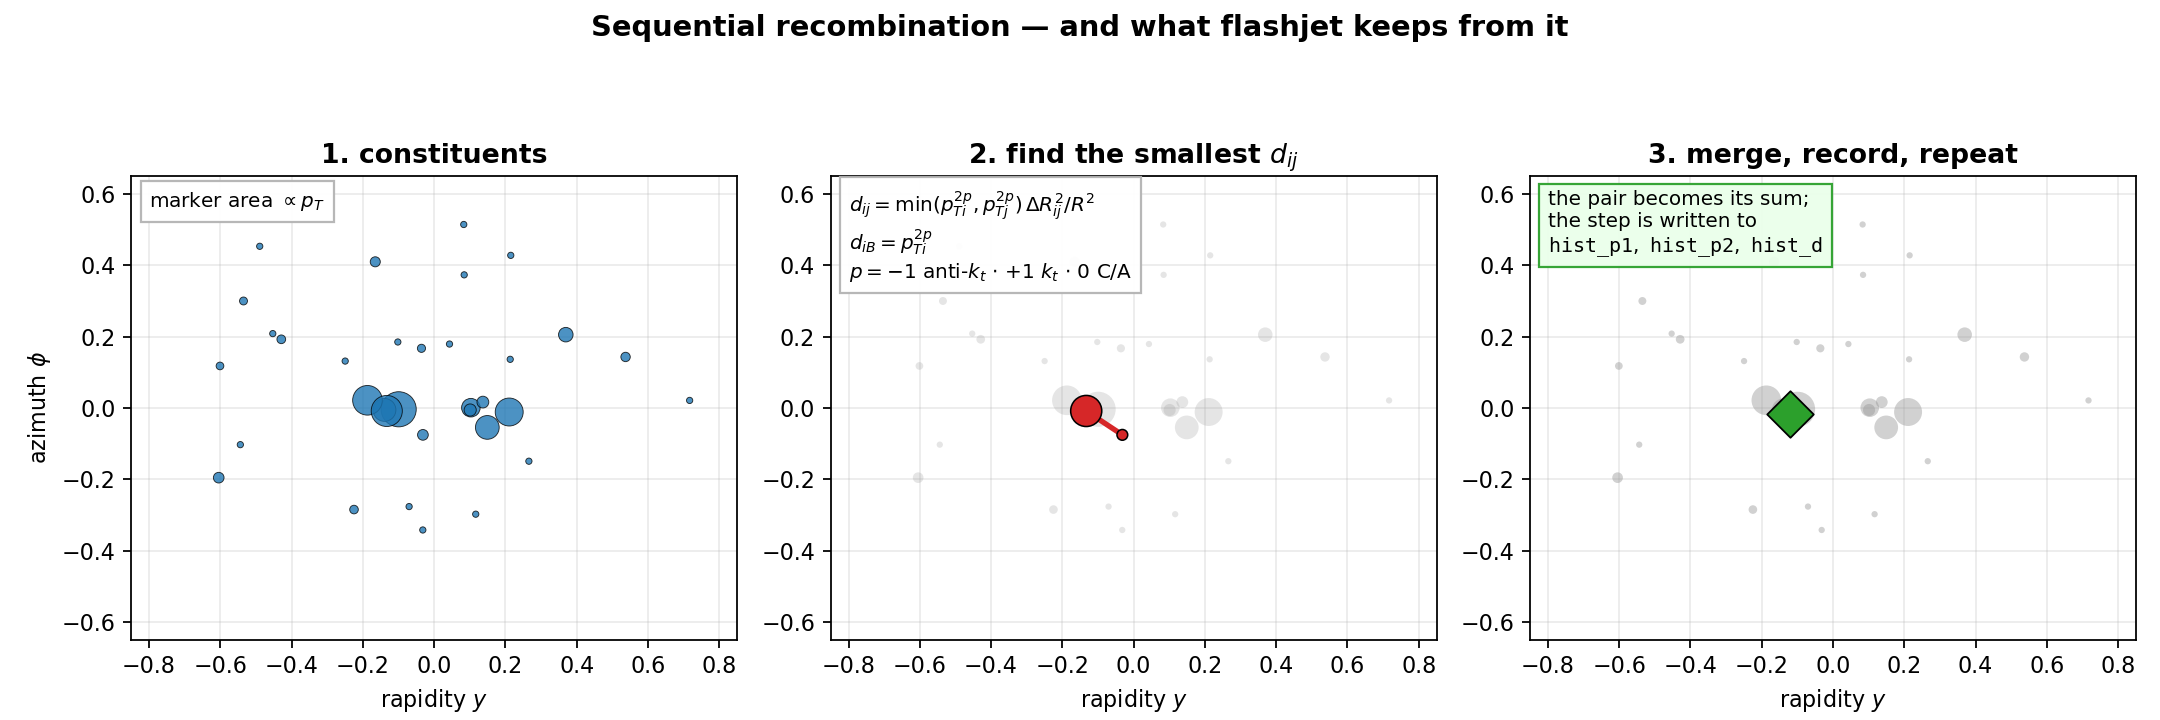
\includegraphics[width=0.95\linewidth]{fig/clustering_steps.png}
\end{center}
\vspace{-0.5em}
\begin{columns}[T]
\begin{column}{0.52\textwidth}
\small
\textbf{Two distances, computed for every pair:}
\begin{itemize}\setlength\itemsep{0.15em}
  \item $d_{ij}$ --- \emph{pair} distance, particle $i$ to particle $j$
  \item $d_{iB}$ --- \emph{beam} distance, particle $i$ to the beam
\end{itemize}
\end{column}
\begin{column}{0.48\textwidth}
\small
\textbf{Then repeat until nothing is left:}
\begin{enumerate}\setlength\itemsep{0.15em}
  \item find the smallest of all distances
  \item if it is a $d_{ij}$: \textbf{merge} $i$ and $j$
  \item if it is a $d_{iB}$: call $i$ a \textbf{jet}, remove it
\end{enumerate}
\end{column}
\end{columns}
\smallnote{Both distances were defined on the previous slide; the exponent $p$
there selects which algorithm this loop runs.}
\end{frame}

\begin{frame}{\akt{} gives rigid, circular jets \hfill \toyB}
\begin{center}
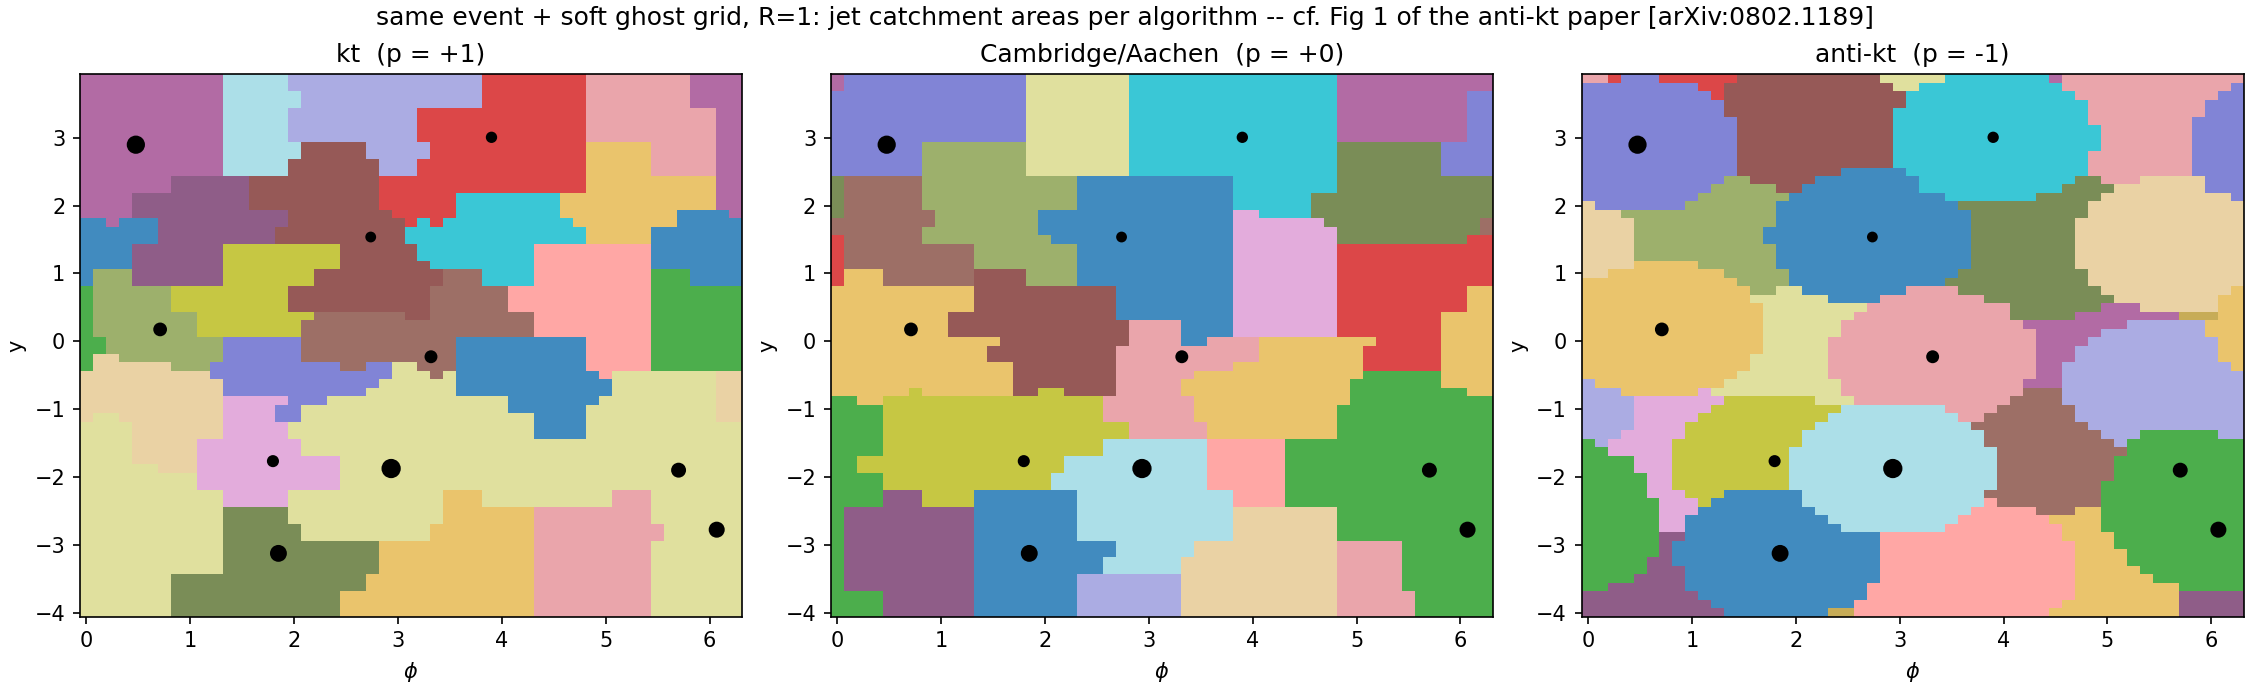
\includegraphics[width=0.93\linewidth]{fig/jet_areas.png}
\end{center}
\vspace{-0.4em}
\begin{columns}[T]
\begin{column}{0.48\textwidth}
\small
\begin{itemize}\setlength\itemsep{0.1em}
  \item jet catchment areas, all three algorithms
  \item clustered by \textbf{flashjet itself}
\end{itemize}
\end{column}
\begin{column}{0.52\textwidth}
\small
\begin{itemize}\setlength\itemsep{0.1em}
  \item $k_t$, C/A: \textbf{ragged}, fluctuating boundaries
  \item \akt: \textbf{circles of area $\pi R^2$} on each hard particle
  \item[$\Rightarrow$] the algorithm's defining result, \textbf{reproduced
        without FastJet}
\end{itemize}
\end{column}
\end{columns}
\end{frame}

\begin{frame}{It returns the tree, not just the jets}
Clustering a batch returns \textbf{two} things --- the jets, and the record of how
they were built.
\medskip

\begin{center}
\small
\begin{tabular}{@{}lll@{}}
\toprule
\textbf{field} & \textbf{shape} & \textbf{what it holds}\\
\midrule
\texttt{jet\_idx} & $(B,N)$ & which jet each particle ended up in\\
\texttt{n\_jets} & $(B,)$ & how many jets were found\\
\addlinespace
\texttt{hist\_p1}, \texttt{hist\_p2} & $(B,N)$ & \textbf{which pair merged}, at each step\\
\texttt{hist\_child} & $(B,N)$ & what they merged \emph{into}\\
\texttt{hist\_d} & $(B,N)$ & the distance $d_{ij}$ at that step\\
\bottomrule
\end{tabular}
\end{center}
\medskip

\begin{block}{The tree is the product, not a by-product}
\small The bottom three rows are the \textbf{complete binary merge tree}. Groomed
mass, $z_g$, $R_g$, Lund coordinates and exclusive subjets are not separate
algorithms --- they are \textbf{coordinates on that one tree}. Compute it once,
read them all off, \textbf{no second clustering pass}.
\end{block}
\vspace{0.2em}
\begin{center}
\small\color{fjgray} Three things are read off that tree --- F1, F2, F3 --- and then
we look at it on a real jet.
\end{center}
\end{frame}

\begin{frame}{What is implemented}
\begin{columns}[T]
\begin{column}{0.5\textwidth}
\textbf{Clustering}
\begin{itemize}
  \item generalised-$k_t$: \akt, $k_t$, C/A
  \item merge history recorded in-kernel
  \item many jets clustered in one batched call
  \item scales from single jets to whole events
\end{itemize}
\end{column}
\begin{column}{0.5\textwidth}
\textbf{Substructure} --- reads of the history
\begin{itemize}
  \item \textbf{F1} exclusive $k_t$ subjets
  \item \textbf{F2} soft drop / mMDT / mass-drop
  \item \textbf{F3} primary Lund coordinates
\end{itemize}
\smallskip
\smallnote{All three are pure-torch post-reads: no kernel changes, CPU/GPU
identical, negligible cost.}
\end{column}
\end{columns}
\end{frame}

% ------------------------------------------------------------
\begin{frame}{F1 --- exclusive subjets from the $k_t$ history \hfill \toyA}
\begin{columns}[T]
\begin{column}{0.42\textwidth}
\textbf{What it does.} Undo the last merges of the sequence to expose exactly
$n$ subjets --- or stop at a $d_{cut}$.
\smallskip

\textbf{How.} The history is already a binary tree. Walk back up it $n-1$ steps;
no reclustering.
\smallskip

\textbf{Why $k_t$.} $k_t$ merges the softest pair first, so the \emph{last}
merges are the hard prongs --- exactly what a 2-prong decay leaves behind.
\smallskip

The splitting scales come straight from \texttt{hist\_d}:
\[\sqrt{d_{12}},\ \sqrt{d_{23}},\ \dots\]
\vspace{-1.0em}
\[\text{with}\ \ d_{ij}=\min\!\left(p_{Ti}^{2},p_{Tj}^{2}\right)\frac{\Delta R_{ij}^2}{R^2}\]
\end{column}
\begin{column}{0.58\textwidth}
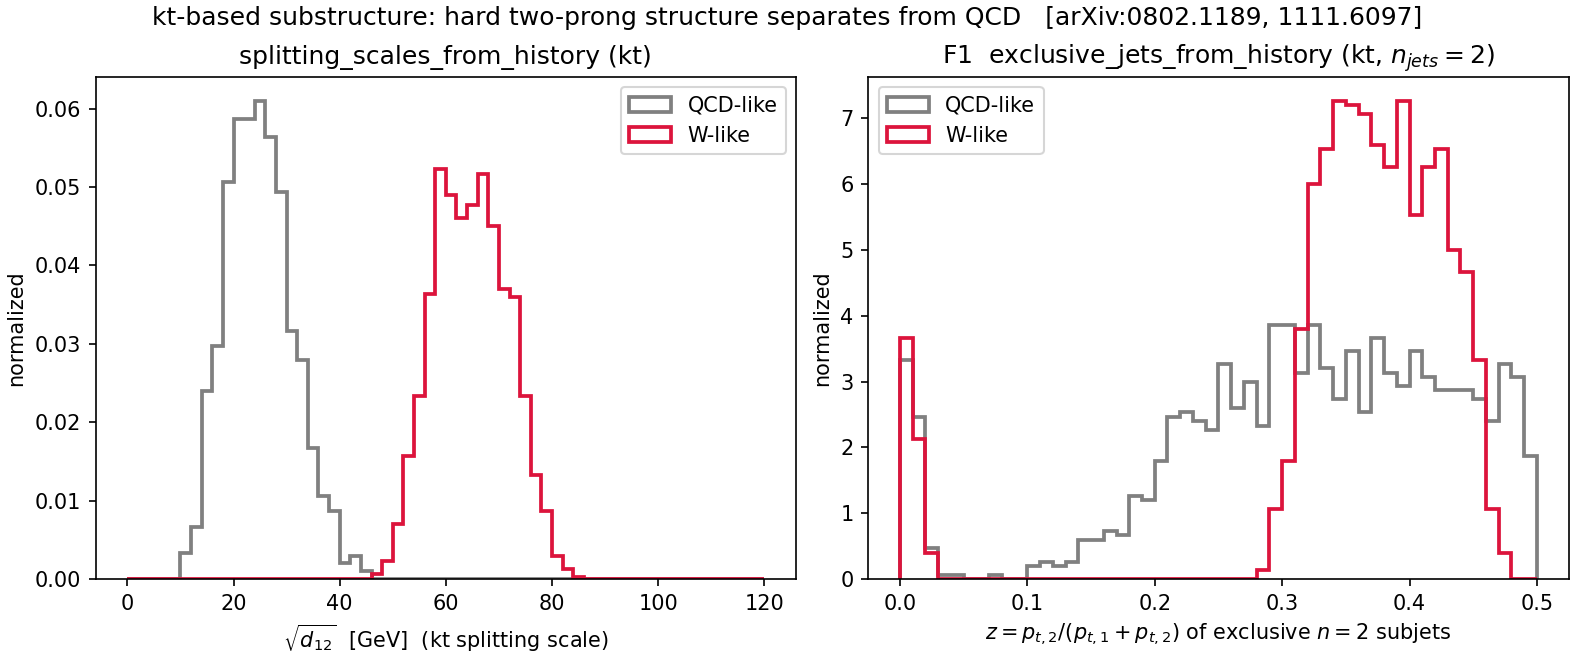
\includegraphics[width=\linewidth]{fig/kt_observables.png}\\
\smallnote{Toy W-like (2-prong) vs QCD-like fat jets.
\textbf{Left:} the $k_t$ splitting scale $\sqrt{d_{12}}$ separates cleanly.
\textbf{Right:} the momentum balance $z$ of the two exclusive subjets ---
the W sits near $z \sim 0.4$, QCD spreads to small~$z$.}
\end{column}
\end{columns}
\end{frame}

% ------------------------------------------------------------
\begin{frame}{F2 --- soft drop / mMDT grooming \hfill \toyA}
\begin{center}
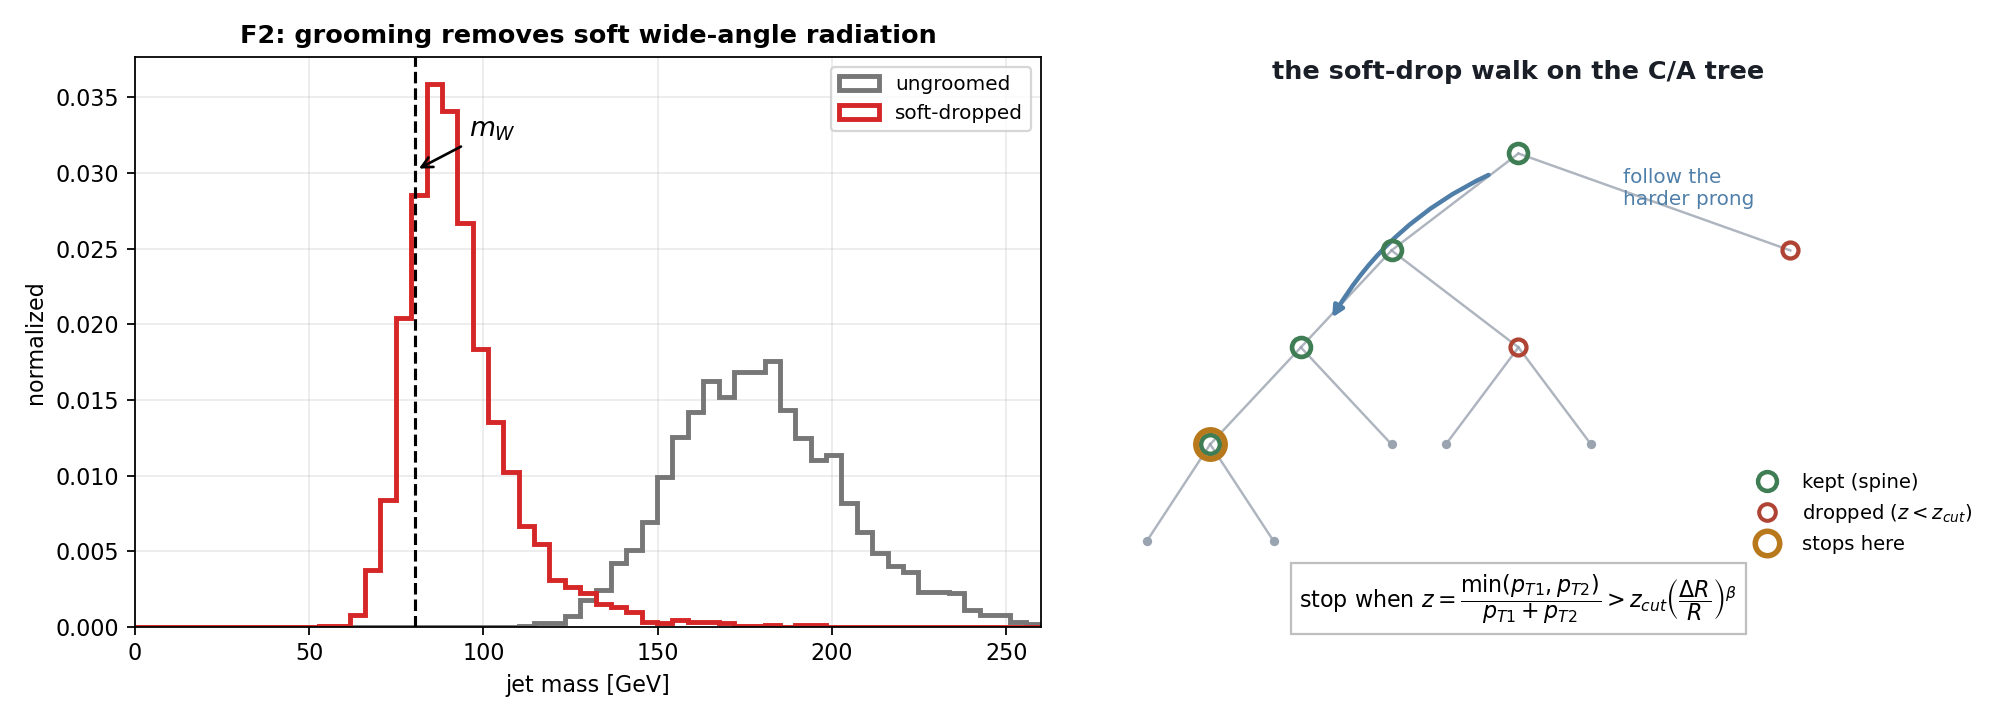
\includegraphics[width=0.88\linewidth]{fig/softdrop_walk.png}
\end{center}
\vspace{-0.2em}
\begin{center}
\textbf{Stop when}\quad
$\displaystyle
\frac{\min(p_{T1},p_{T2})}{p_{T1}+p_{T2}}
\;>\; z_{\mathrm{cut}}\left(\frac{\Delta R_{12}}{R}\right)^{\beta}$
\end{center}
\vspace{0.1em}
\begin{columns}[T]
\begin{column}{0.5\textwidth}
\smallnote{Walk down the C/A tree along the harder branch, discarding the softer
prong until that condition is met. $\beta=0$ recovers mMDT.}
\end{column}
\begin{column}{0.5\textwidth}
\smallnote{The walk is $O(\log_2 n)$ on the stored tree --- it never touches the
constituents again, so grooming is essentially free once clustered.}
\end{column}
\end{columns}
\end{frame}

% ------------------------------------------------------------
\begin{frame}{What the tree looks like on real jets \hfill \realC}
\begin{center}
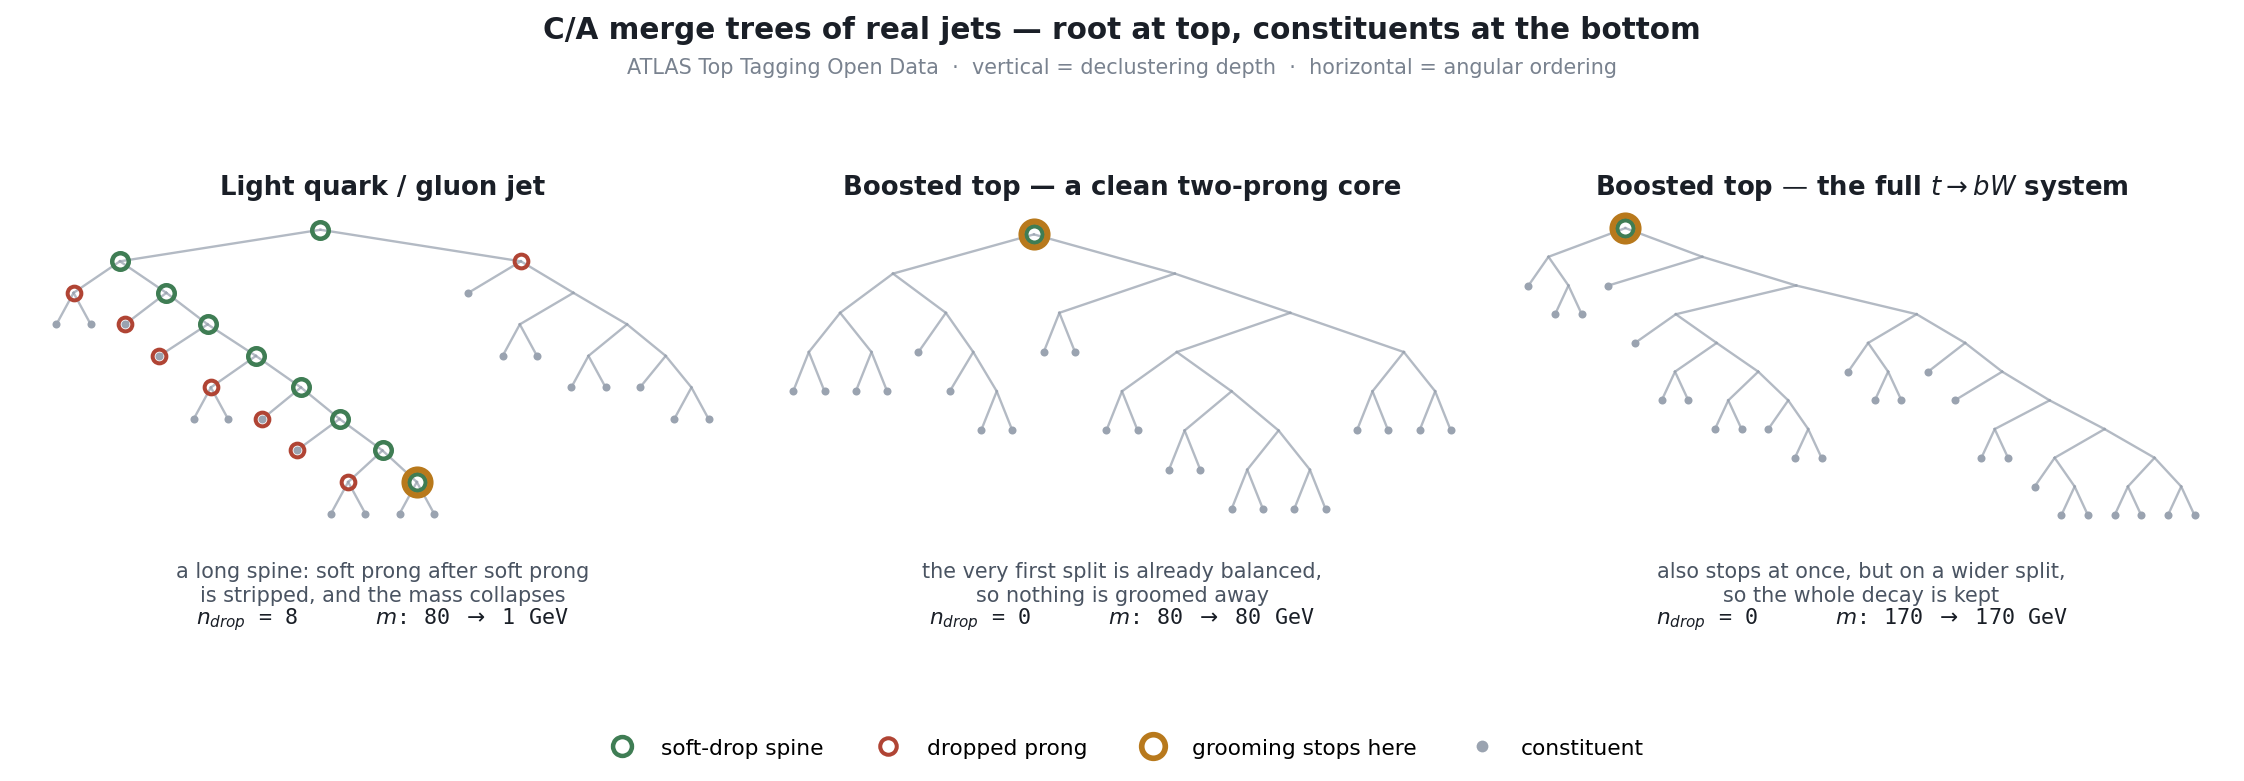
\includegraphics[width=0.97\linewidth]{fig/tree_gallery.png}
\end{center}
\vspace{-0.5em}
\begin{columns}[T]
\begin{column}{0.5\textwidth}
\smallnote{\textbf{A jet without a decay has nothing to stop on.} The
light-quark/gluon jet is a long \emph{staircase}: soft prong after soft prong is
stripped, and its mass collapses to nothing.}
\end{column}
\begin{column}{0.5\textwidth}
\smallnote{\textbf{A real decay stops at once.} Both top jets halt on their very
first split, because it is already hard and balanced --- so the mass survives.}
\end{column}
\end{columns}
\smallskip
\smallnote{ATLAS Open Data, C/A with soft drop ($z_{cut}\!=\!0.1$, $\beta\!=\!0$).
\textbf{The number of drops is itself a discriminant} --- and it is read straight
off the stored tree, at no extra cost.}
\end{frame}

\begin{frame}{F3 --- primary Lund coordinates \hfill \toyA}
\begin{center}
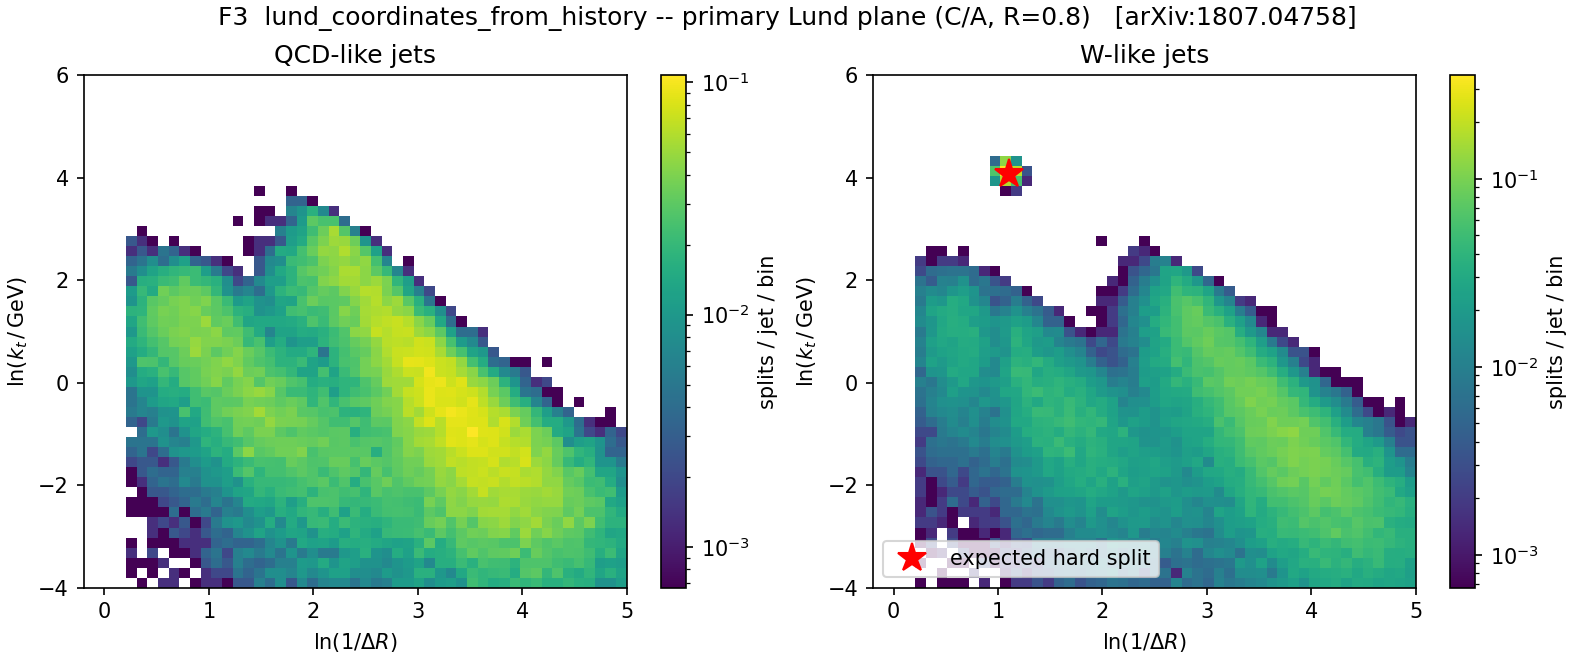
\includegraphics[width=0.80\linewidth]{fig/lund_plane.png}
\end{center}
\vspace{-0.6em}
\begin{columns}[T]
\begin{column}{0.34\textwidth}
\smallnote{\textbf{What.} Every primary splitting emits
$z=\tfrac{p_{T2}}{p_{T1}+p_{T2}}$, $\Delta R$, $k_t=p_{T2}\Delta R$, and the
plane coordinates $\big(\ln\tfrac{1}{\Delta R},\ \ln k_t\big)$.}
\end{column}
\begin{column}{0.32\textwidth}
\smallnote{\textbf{How.} One pass down the primary branch --- each node is one
point in the plane.}
\end{column}
\begin{column}{0.34\textwidth}
\smallnote{\textbf{Check.} The $d$-channel ties \emph{exactly} to the splitting
scales computed independently.}
\end{column}
\end{columns}
\smallnote{QCD fills the soft-collinear region smoothly; the W-like sample adds a
\textbf{localised hard splitting} exactly where the decay is predicted to sit
(star).}
\end{frame}

% ============================================================
\section{Correctness}

\begin{frame}{Closures against analytic predictions \hfill \toyB}
\begin{columns}[T]
\begin{column}{0.5\textwidth}
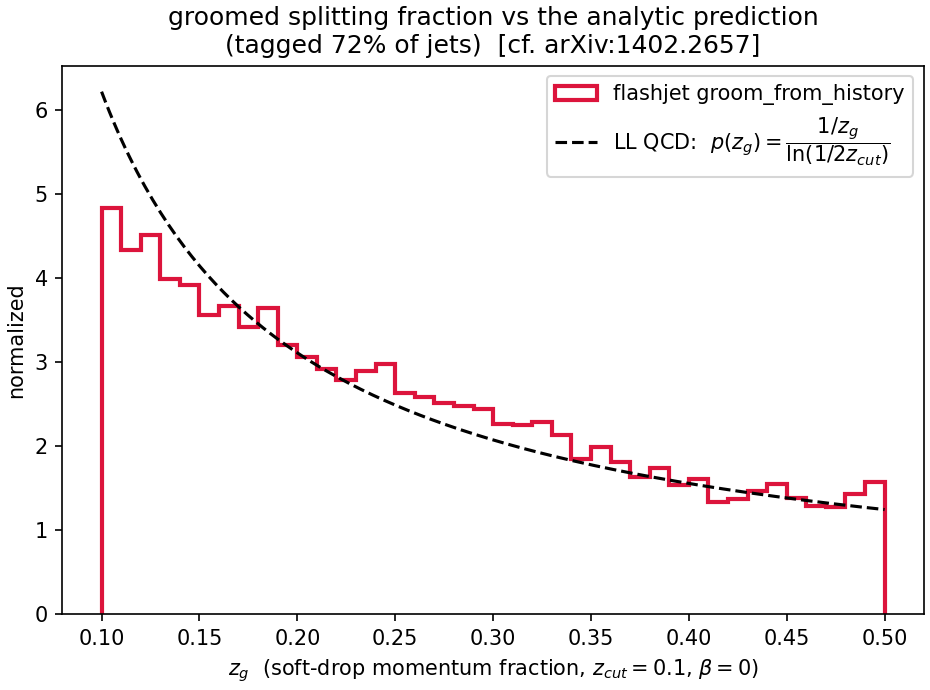
\includegraphics[width=0.93\linewidth]{fig/zg_distribution.png}\\
\smallnote{Soft-drop $z_g$ follows the $1/z$ form predicted at leading-log,
recovered from the C/A history.}
\end{column}
\begin{column}{0.5\textwidth}
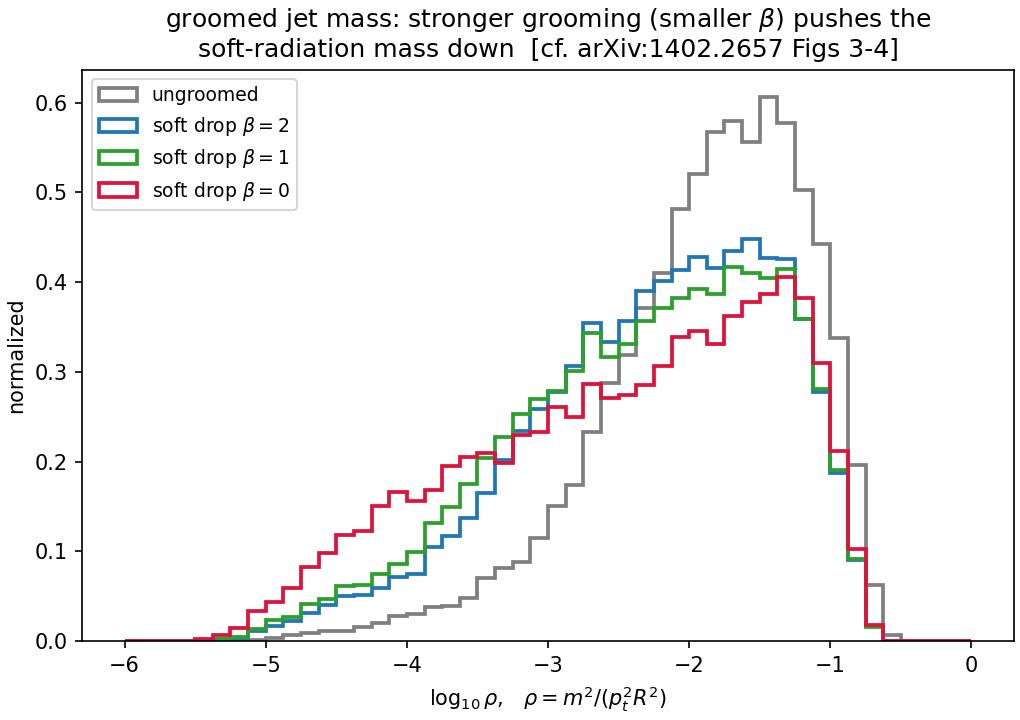
\includegraphics[width=0.93\linewidth]{fig/softdrop_rho.png}\\
\smallnote{Groomed-mass ordering in $\beta$: larger $\beta$ grooms less, so the
mass peak moves up.}
\end{column}
\end{columns}
\smallskip
\smallnote{\textbf{Toys first:} on generated input the answer is known
analytically, so anything off the curve is a real bug. Real-data checks follow.
Toy-shower input tests the decoders, not an event generator.}
\end{frame}

\begin{frame}{Jet by jet, against ATLAS's own stored values \hfill \realC}
\begin{center}
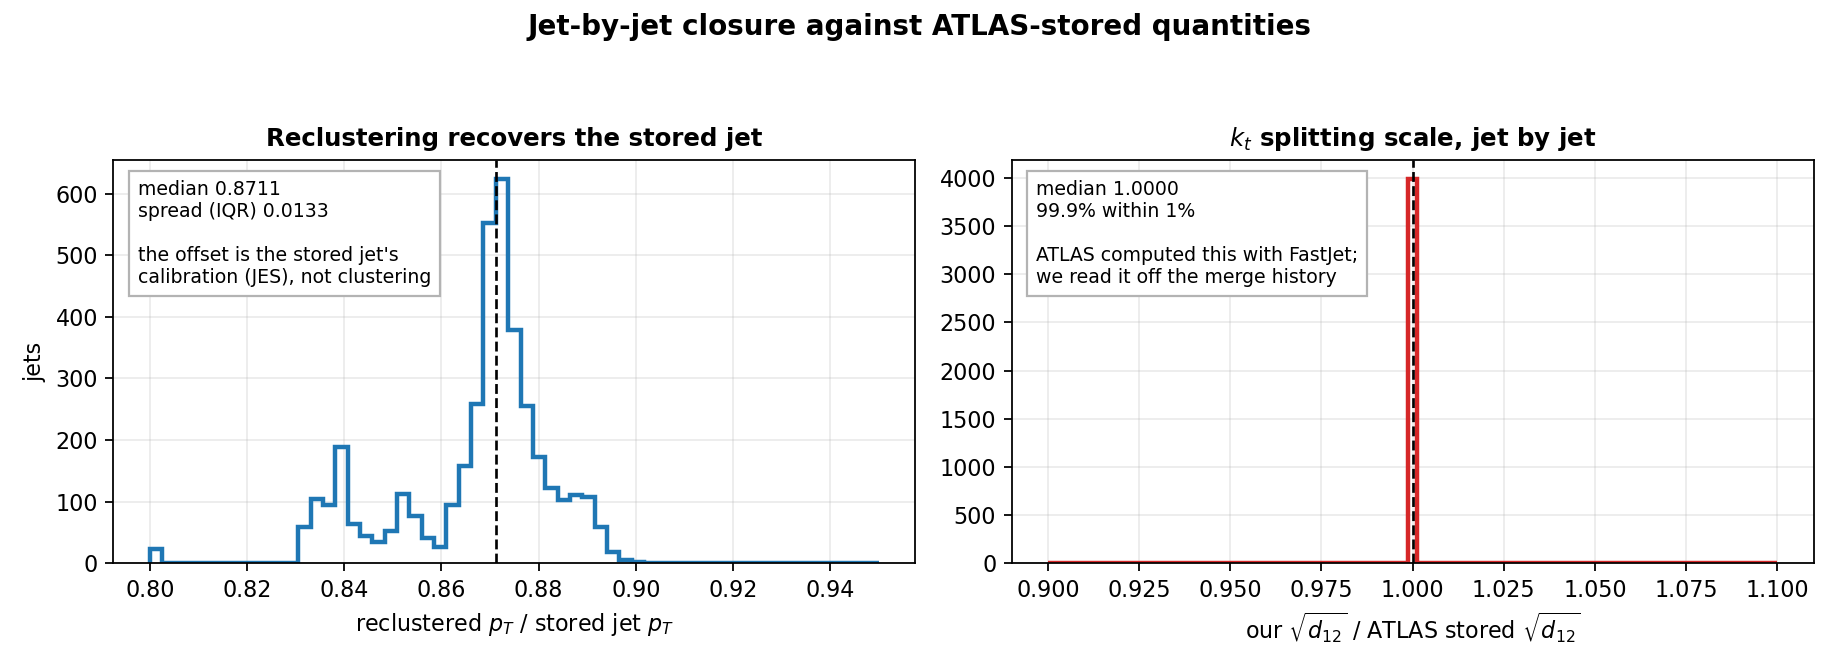
\includegraphics[width=0.92\linewidth]{fig/atlas_jetbyjet.png}
\end{center}
\vspace{-0.4em}
\begin{columns}[T]
\begin{column}{0.5\textwidth}
\smallnote{\textbf{Left.} Reclustering the stored constituents recovers the
stored jet with a \textbf{0.013 spread}. The 0.87 offset is the stored jet's
\textbf{calibration}, applied after clustering --- it is present before we touch
anything.}
\end{column}
\begin{column}{0.5\textwidth}
\smallnote{\textbf{Right.} The $k_t$ splitting scale $\sqrt{d_{12}}$ against the
value \textbf{ATLAS computed with FastJet} and stored: median \textbf{1.0000},
\textbf{99.9\,\%} within 1\,\%. We read ours straight off the merge history.}
\end{column}
\end{columns}
\end{frame}

\begin{frame}{It gives the same jets --- everywhere we looked \hfill \realC}
\begin{columns}[T]
\begin{column}{0.52\textwidth}
\begin{block}{vs FastJet --- a 150-point grid}
\small 3 algorithms $\times$ 5 radii $\times$ 5 multiplicity bins $\times$ 2
samples, 20\,000 jets each.
\smallskip

\textbf{100.000\,\%} jet-count agreement at \textbf{every} point.
\end{block}
\smallnote{Leading-jet $p_T$ within $10^{-4}$ at 148/150; median difference
$\sim7\times10^{-8}$ --- float32 precision.}
\end{column}
\begin{column}{0.48\textwidth}
\begin{block}{vs ATLAS's own reconstructed jets}
\small Cluster the $\sim$600 stored calorimeter clusters ourselves; compare to
the jets ATLAS reconstructed and published.
\smallskip

\textbf{100.0\,\%} $n_{\rm jets}$ match, \textbf{10.96 vs 10.96} jets/event.
\end{block}
\smallnote{The event regime, where the problem is $O(N^2)$.}
\end{column}
\end{columns}
\vspace{0.3em}

\begin{block}{}
\small Two \emph{independent} references: FastJet for the jets, a separate
\textbf{NumPy tree-walk} for every substructure decoder. The second test closes
the algorithm against \textbf{the experiment's published output} --- not against
another implementation of the same algorithm.
\end{block}
\smallnote{Per-point tables and the $R$/multiplicity scans are in backup.}
\end{frame}

% ============================================================
\section{Speed --- the jet regime}

\begin{frame}{The benchmark --- jet regime \hfill \realC}
\begin{columns}[T]
\begin{column}{0.5\textwidth}
\textbf{Data} --- ATLAS Open Data, freely presentable

\smallskip
\begin{tabular}{@{}lrr@{}}
\toprule
sample & jets & $\langle n_{\rm const}\rangle$\\
\midrule
boosted top & 30\,000 & 59.2\\
QCD (light $q/g$) & 30\,000 & 52.4\\
\bottomrule
\end{tabular}
\smallskip

\smallnote{Large-$R$ jets with calorimeter-cluster constituents. The grid is
\textbf{3 algorithms $\times$ 5 radii $\times$ 5 multiplicity bins}, 20\,000 jets
per bin.}
\end{column}
\begin{column}{0.5\textwidth}
\textbf{Method}
\begin{enumerate}
  \item extract constituents once, save;
  \item cluster on GPU, time it, save the \emph{same} events;
  \item cluster those saved events with FastJet;
  \item \textbf{check they agree} --- else the timing is meaningless.
\end{enumerate}
\smallskip
\begin{block}{}
\small Both clusterers read the \textbf{same saved file}. Speedups are quoted
against the \textbf{vectorised} FastJet interface --- the faster, fairer baseline.
\end{block}
\smallnote{\textbf{One timed unit = one large-$R$ jet} (24--123 constituents),
batched. Event-regime timing is not in this talk.}
\end{column}
\end{columns}
\end{frame}

\begin{frame}{Time per jet --- jet regime \hfill \realC}
\begin{center}
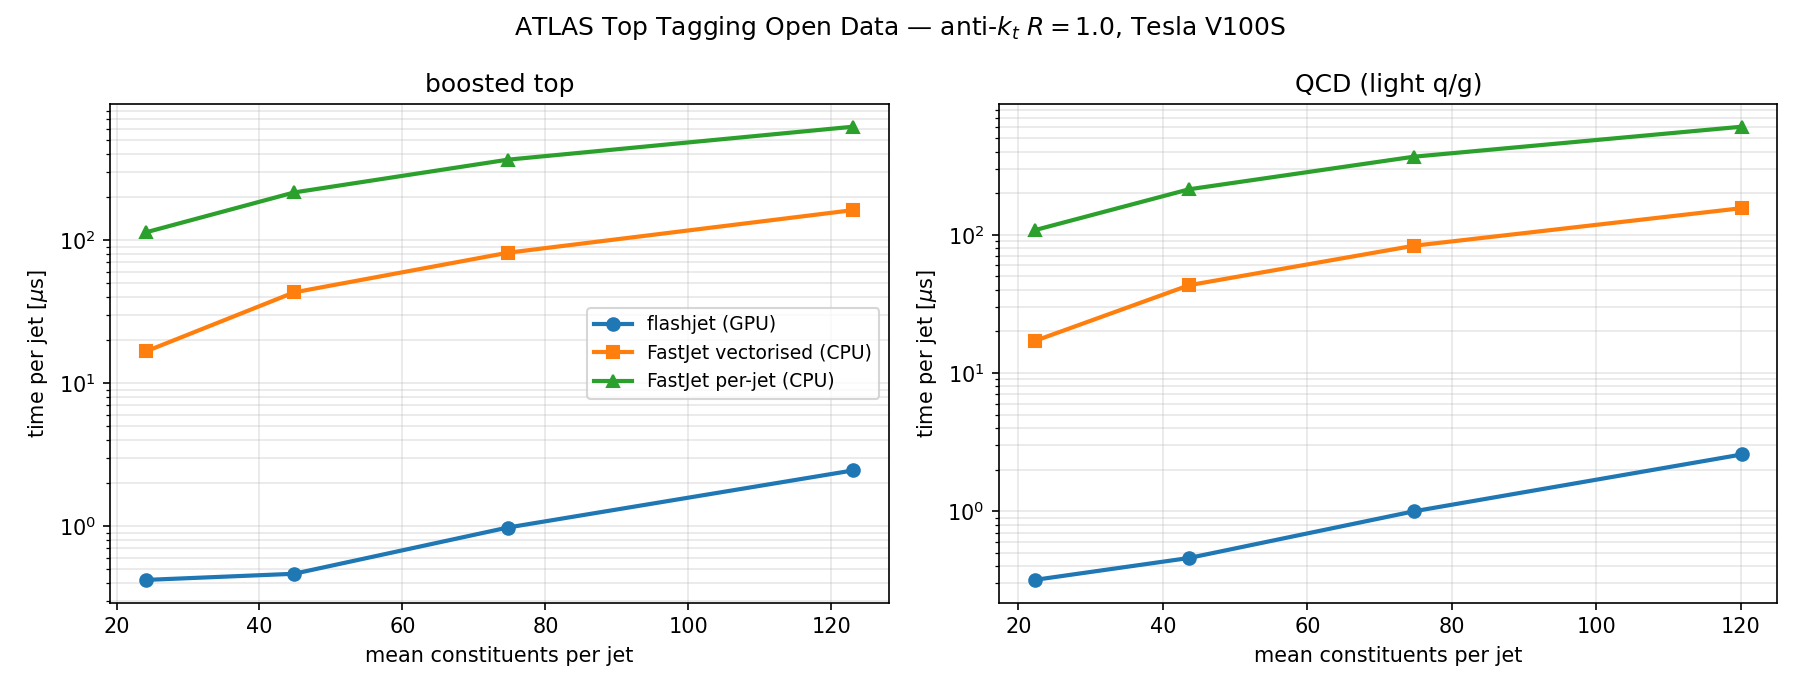
\includegraphics[width=0.90\linewidth]{fig/atlas_abs_timing.png}
\end{center}
\smallnote{\textbf{Log scale} --- each gridline is $10\times$. flashjet stays
nearly flat while both FastJet interfaces climb steeply with multiplicity:
\textbf{0.35--2.7\,$\mu$s per jet} against \textbf{17--155\,$\mu$s} for vectorised
FastJet, and \textbf{110--620\,$\mu$s} per jet one at a time. Benchmarked on an
NVIDIA \textbf{V100-class} GPU. \textbf{Per jet, batched} --- the GPU clusters the
whole batch at once, so this is amortised cost, not single-jet latency.}
\end{frame}

\begin{frame}{The advantage grows with jet complexity --- jet regime \hfill \realC}
\begin{center}
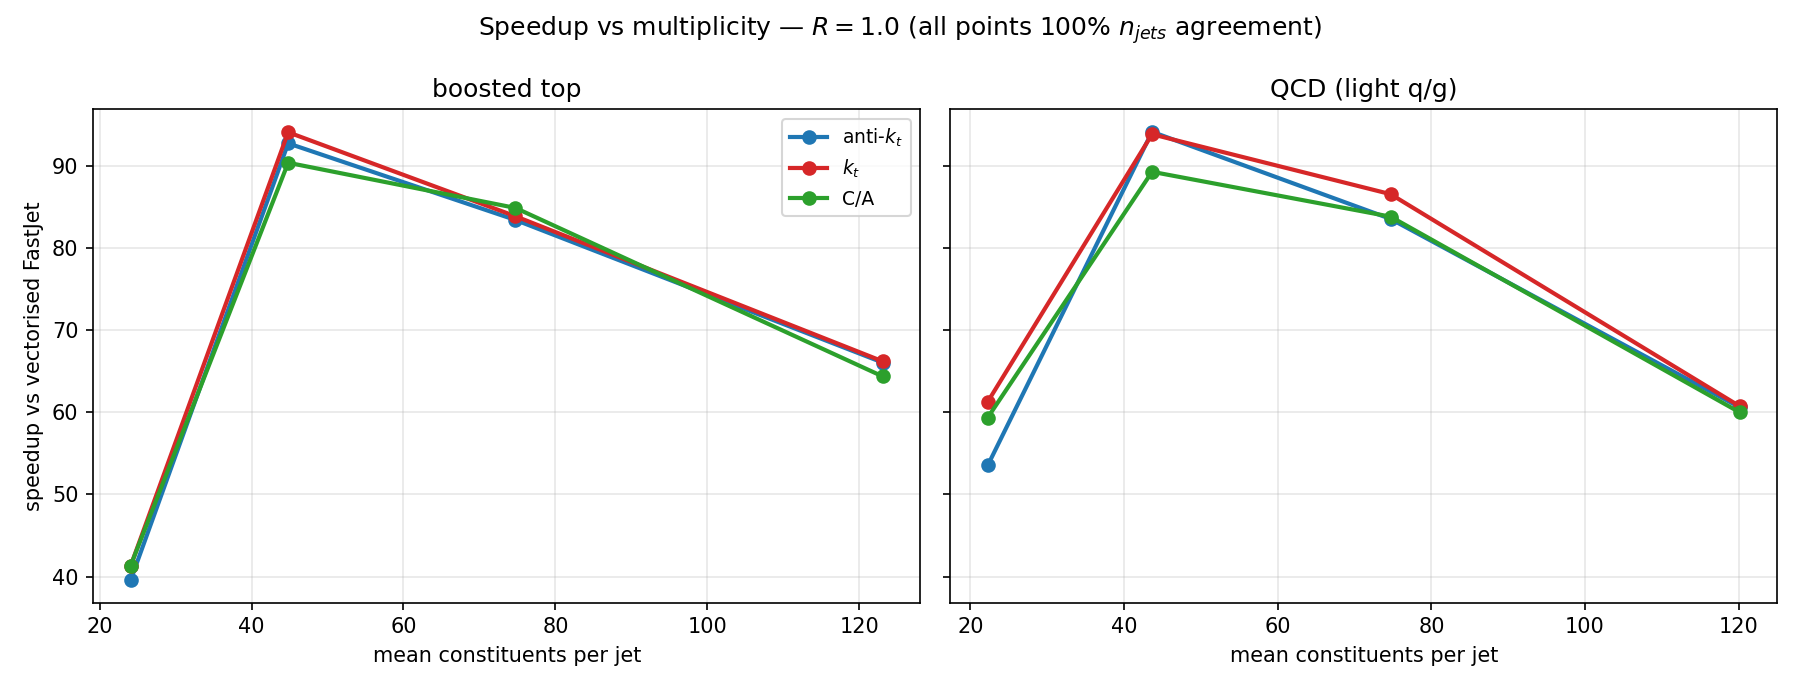
\includegraphics[width=0.90\linewidth]{fig/atlas_speedup_algs.png}
\end{center}
\smallnote{All three algorithms, both samples, $R=1.0$. \textbf{39--99$\times$}
over vectorised FastJet across the grid (median \textbf{64$\times$}), and every
point has \textbf{100\,\%} $n_{\rm jets}$ agreement. Busier jets $\rightarrow$
bigger win --- the regime that matters for boosted-object physics.}
\end{frame}

\begin{frame}[fragile]{Using it}
\begin{Verbatim}[fontsize=\footnotesize,frame=single,rulecolor=\color{fjgray}]
import flashjet

out = flashjet.cluster(p4, mask, R=1.0, algorithm="antikt")
\end{Verbatim}
\vspace{-0.3em}
{\footnotesize
\begin{tabular}{@{}lll@{}}
\toprule
\textbf{argument} & \textbf{type} & \\
\midrule
\texttt{p4} & $(B,N,4)$ tensor & $(p_x,p_y,p_z,E)$; CPU or CUDA\\
\texttt{mask} & $(B,N)$ bool & marks real constituents in a padded batch\\
\texttt{R} & float & jet radius\\
\texttt{algorithm} & str & \texttt{"antikt"} $\vert$ \texttt{"kt"} $\vert$ \texttt{"cambridge"}\\
\texttt{p} & float & generalised-$k_t$ exponent (overrides \texttt{algorithm})\\
\bottomrule
\end{tabular}}
\medskip

\begin{Verbatim}[fontsize=\footnotesize,frame=single,rulecolor=\color{fjgray}]
out.n_jets                                    # (B,)     jets found
out.jets_p4(p4)                               # (B,J,4)  jet four-momenta
out.splitting_scales()                        #          sqrt(d12), sqrt(d23), ...
out.exclusive_jets(n_jets=3)                  # F1       exclusive kt subjets
out.groomed_jets(p4, R, z_cut=0.1, beta=0.0)  # F2       soft drop / mMDT
out.lund_coordinates(p4, R)                   # F3       primary Lund plane
\end{Verbatim}
\smallnote{The same call runs unchanged on CPU and GPU --- the backend is chosen
from the problem size, not by the caller.}
\end{frame}

% ============================================================
\section{Downstream: the clustering tree as tagger input}

\begin{frame}{Does the tree help a tagger? --- setup}
\begin{columns}[T]
\begin{column}{0.54\textwidth}
\textbf{The question.} Gouskos \& Maier [PLuM, 2605.26821] report that explicit
Lund-plane splittings help a transformer tagger. We test that on a
\textbf{full 10-class} training.
\medskip

\textbf{Model.} Particle Transformer [2202.03772] --- 8 encoder $+$ 2
class-attention blocks, 8 heads, embed 128; \textbf{2.144\,M} parameters.
\medskip

\textbf{Data.} JetClass, 10 classes, 100\,M training jets,
$\sim$\textbf{20.05\,M} test jets, 128 particles/jet.
\medskip

\textbf{Training.} Ranger, lr $10^{-3}$, batch 512, \textbf{$10^{6}$ iterations}
to convergence. All arms read \textbf{identical shards} in the same order;
features are computed \textbf{live} by flashjet inside the loop.
\end{column}
\begin{column}{0.46\textwidth}
\begin{block}{Our baseline reproduces the paper}
\small
\begin{tabular}{@{}lrr@{}}
\toprule
& ours & published\\
\midrule
test accuracy & \textbf{86.21\,\%} & $\sim$86.1\,\%\\
parameters & 2{,}193{,}930 & 2.19\,M\\
\bottomrule
\end{tabular}
\smallskip

\small Like-for-like --- so a difference between arms is the \emph{feature},
not a broken baseline.
\end{block}
\smallskip

\smallnote{\textbf{Shown here: PLuM} --- 48 $k_t$-ordered Lund splittings
$[\ln k_t, \ln 1/\Delta R, \ln z]$, concatenated as extra tokens (176 vs 128).
Two other encodings were tried --- \textbf{subjet} ($n$-body mass, $p_T$
fraction, $n_{\rm const}$) and \textbf{CA5} (per-particle C/A branch points);
both null-or-worse (backup). Bootstrap errors, 16--84th pct.
\textbf{One seed per arm.}}
\end{column}
\end{columns}
\end{frame}

\begin{frame}{Both arms train identically}
\begin{columns}[T]
\begin{column}{0.5\textwidth}
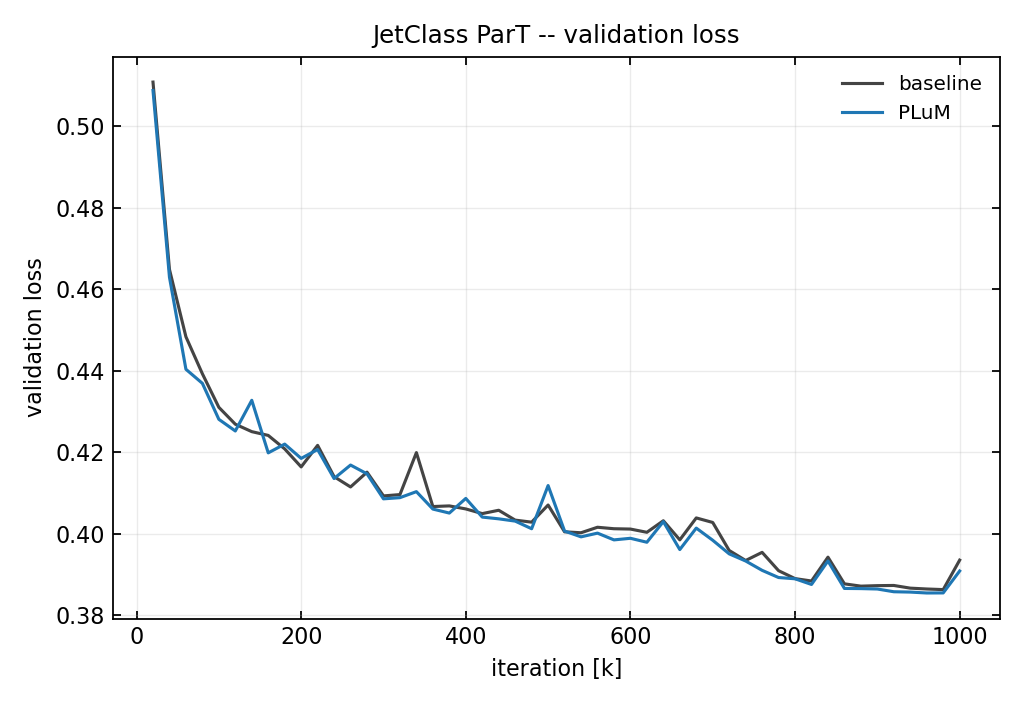
\includegraphics[width=\linewidth]{fig/part_loss_full.png}
\end{column}
\begin{column}{0.5\textwidth}
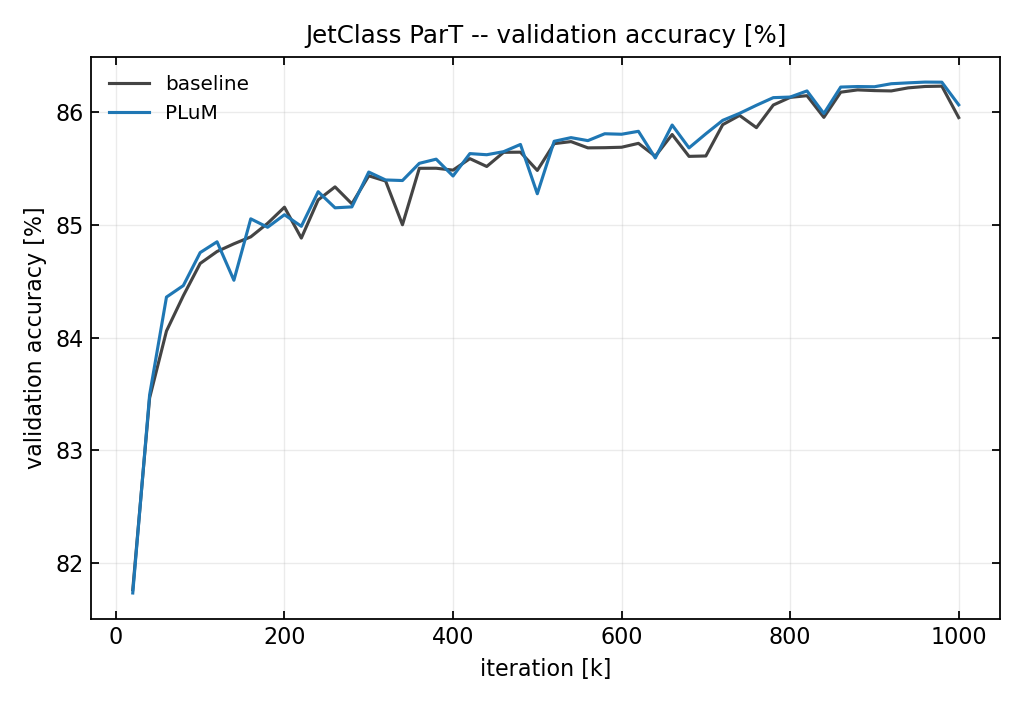
\includegraphics[width=\linewidth]{fig/part_acc_full.png}
\end{column}
\end{columns}
\vspace{-0.2em}
\smallnote{Validation loss and accuracy over the full $10^{6}$ iterations. The
curves are \textbf{on top of each other} --- the feature block does not
destabilise training, and it does not accelerate it either. Both converge to
\textbf{$\sim$86.2\,\%}.}
\end{frame}

\begin{frame}{Top tagging: the gain closes with training \hfill}
\begin{columns}[T]
\begin{column}{0.56\textwidth}
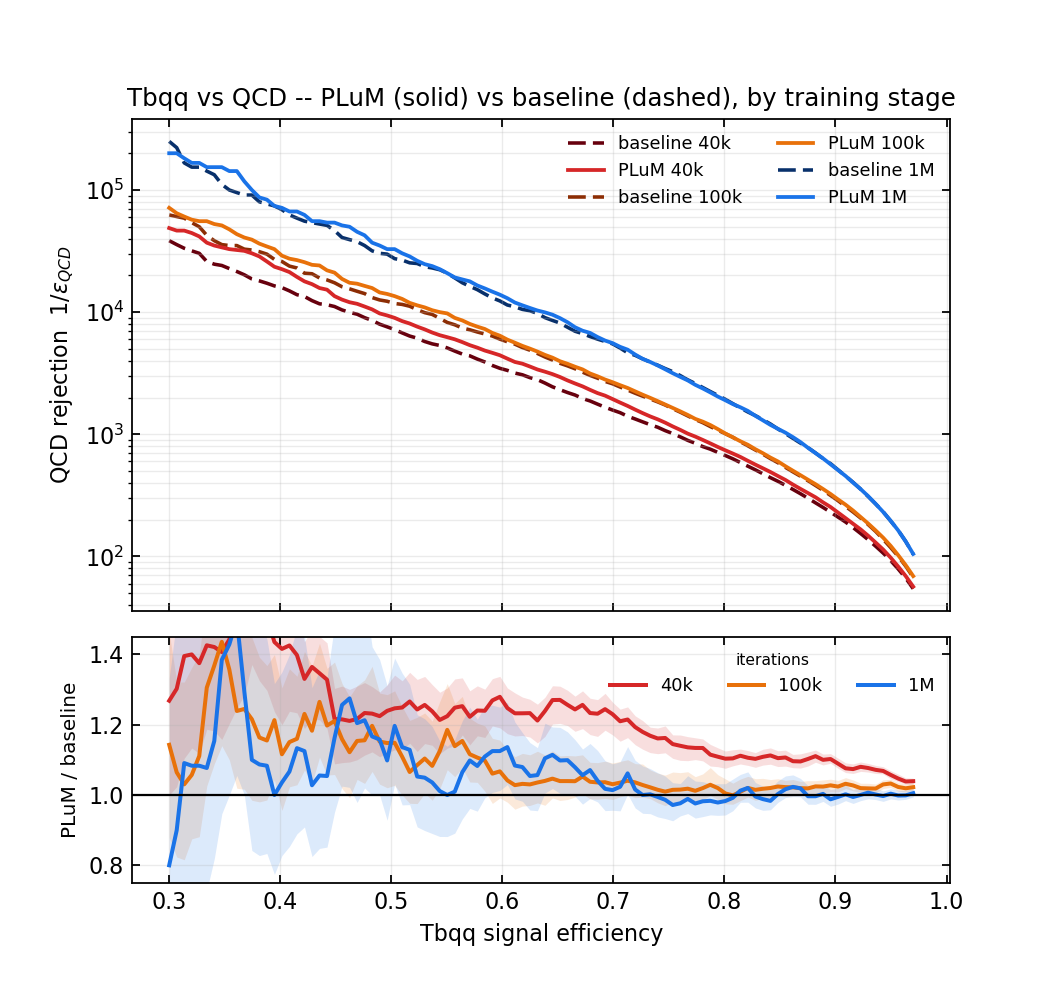
\includegraphics[width=\linewidth,trim=0 18 0 22,clip]{fig/part_rocratio_Tbqq.png}
\end{column}
\begin{column}{0.44\textwidth}
\textbf{$t\rightarrow bqq$ vs QCD.}
\smallskip

Top panel: full ROC at three training stages. Bottom: \textbf{PLuM / baseline}
rejection ratio.
\medskip

\begin{block}{}
\small At \textbf{40k} the ratio sits \textbf{10--25\,\% above 1}. By
\textbf{1M} it has collapsed onto the line.
\end{block}
\smallskip

\smallnote{Bands: unpaired bootstrap of the test set, 16--84th percentile. The
low-efficiency end is noisy because rejection there is $\sim10^{5}$.}
\end{column}
\end{columns}
\end{frame}

\begin{frame}{$H\rightarrow b\bar b$: the paper's best channel \hfill}
\begin{columns}[T]
\begin{column}{0.56\textwidth}
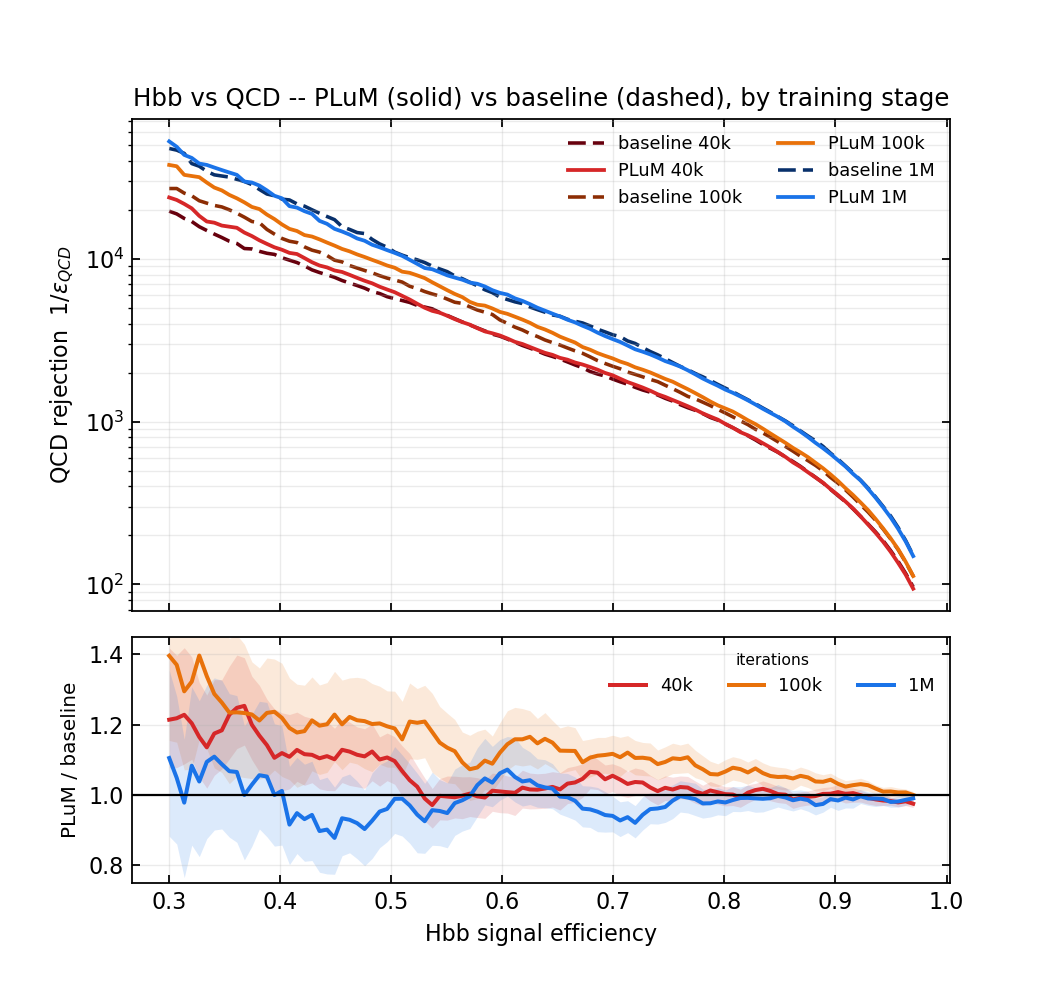
\includegraphics[width=\linewidth,trim=0 18 0 22,clip]{fig/part_rocratio_Hbb.png}
\end{column}
\begin{column}{0.44\textwidth}
\textbf{$H\rightarrow b\bar b$ vs QCD} --- where PLuM report their largest gain.
\smallskip

\begin{block}{}
\small We \textbf{reproduce it early}: $+20\,\%$ at 100k. At \textbf{1M} the
ratio is \textbf{at or below 1}.
\end{block}
\medskip

\smallnote{Their result is obtained in \emph{binary} mode on a fast simulation
\textbf{without secondary-vertex inputs}; ours is a 10-class training. The
early-training agreement is real --- the disagreement is about what survives to
convergence.}
\end{column}
\end{columns}
\end{frame}

\begin{frame}{All seven signal classes --- the same story}
\begin{columns}[T]
\begin{column}{0.68\textwidth}
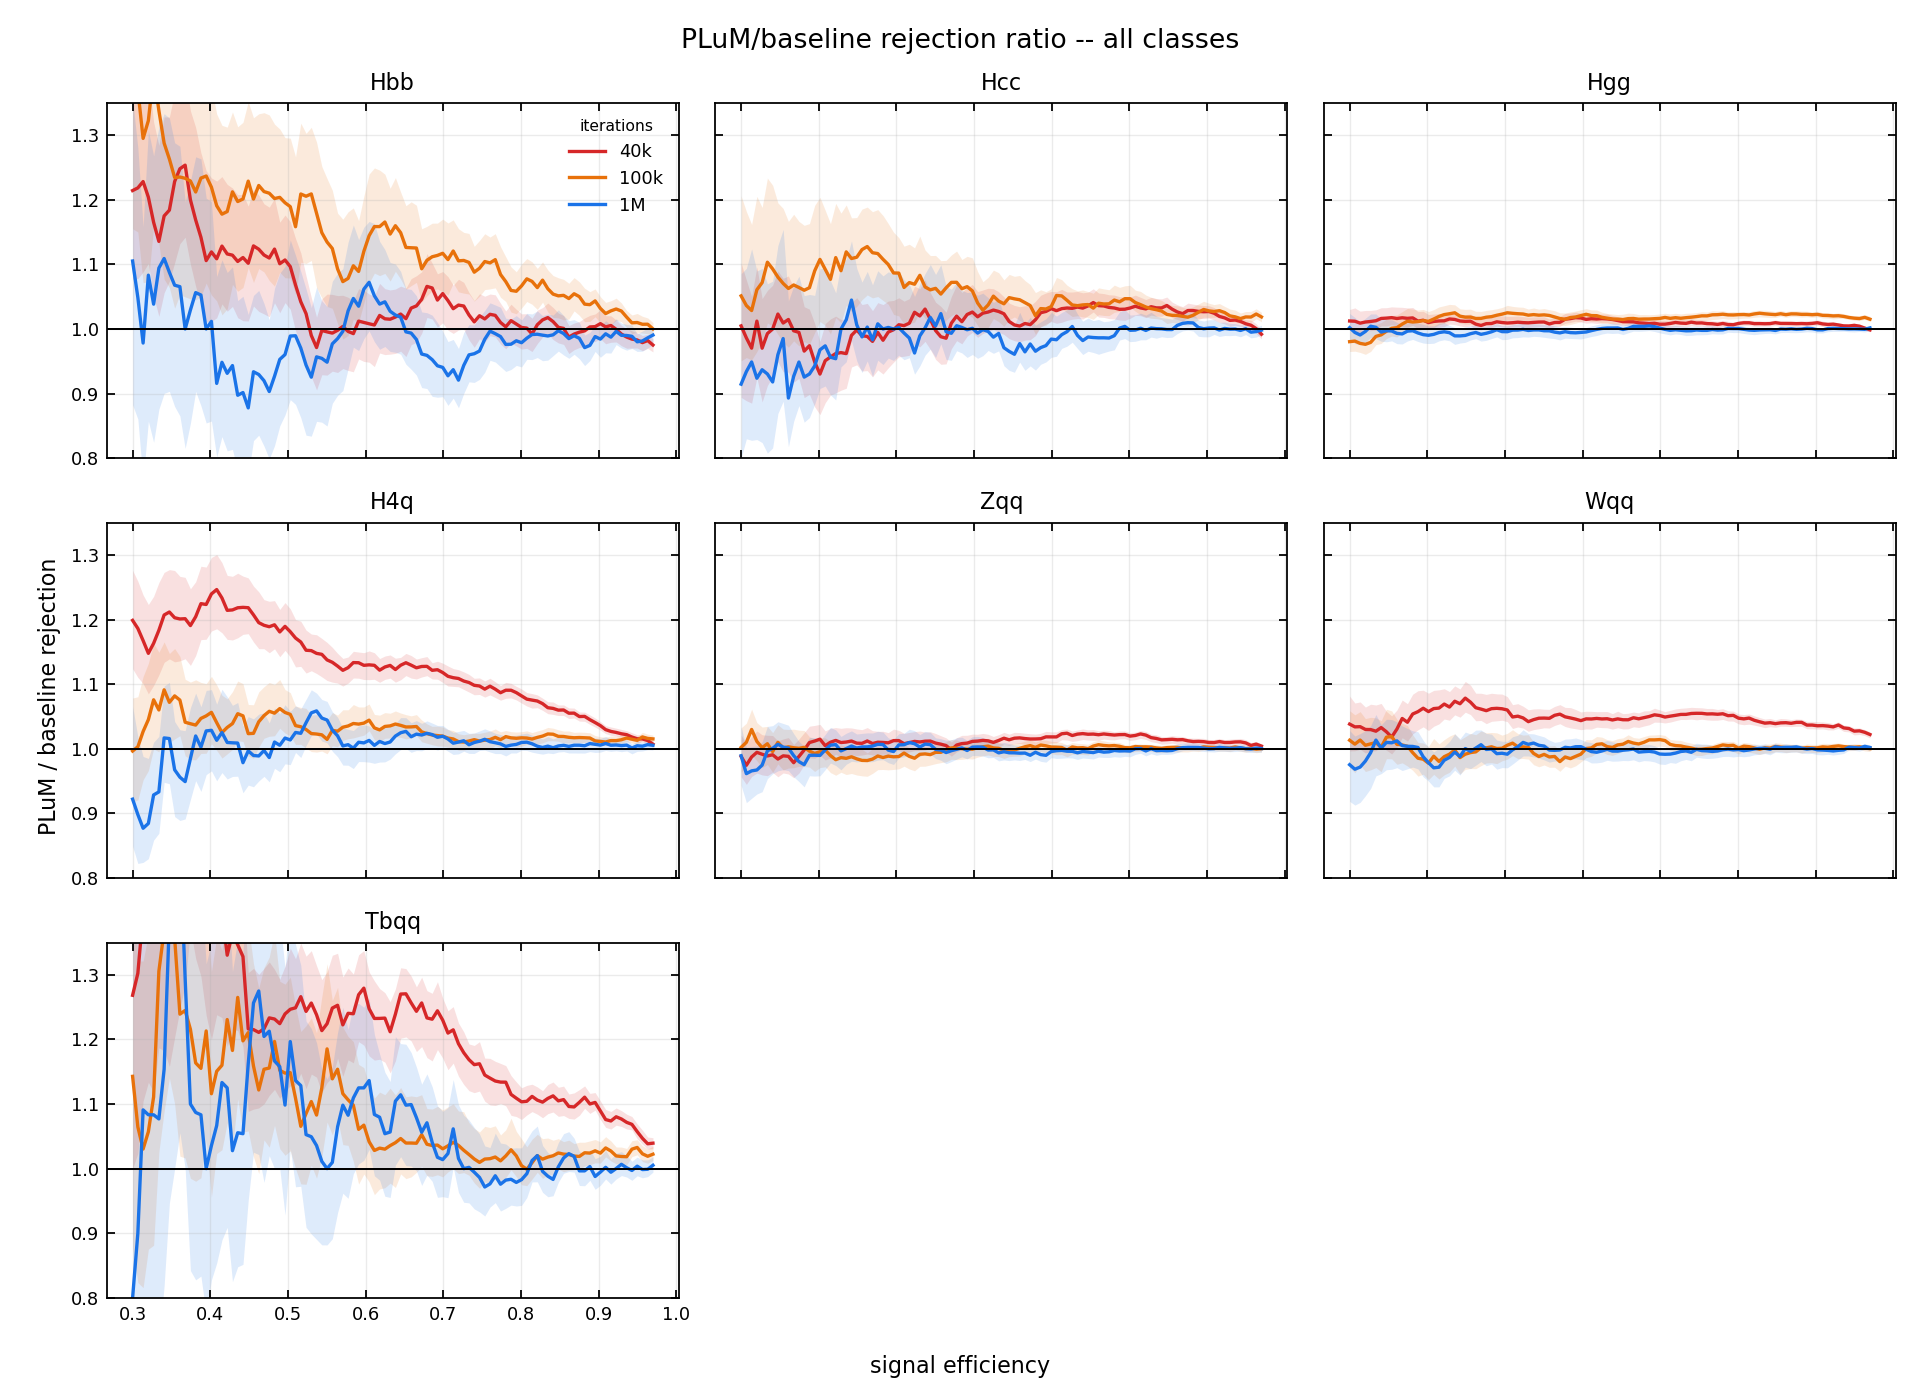
\includegraphics[width=\linewidth,trim=0 55 0 18,clip]{fig/part_ratio_allclasses.png}\\[-0.4em]
\smallnote{PLuM/baseline rejection ratio; unpaired-bootstrap bands.}
\end{column}
\begin{column}{0.32\textwidth}
\textbf{Test accuracy} \smallnote{$\sim$20.05\,M jets}

\scriptsize
\begin{tabular}{@{}lccc@{}}
\toprule
 & 40k & 100k & 1M\\
\midrule
baseline & 83.431 & 84.632 & \textbf{86.212}\\
PLuM & 83.428 & 84.697 & 86.206\\
$\Delta$ & $-0.003$ & $+0.065$ & $-0.006$\\
\bottomrule
\end{tabular}
\smallskip
\begin{block}{What we see}
\scriptsize An \textbf{early gain in every class}, \textbf{gone by 1\,M}. Even
Wqq --- the \emph{fewest} splittings --- gains at $\sim$9$\sigma$ early:
\textbf{not confined to complex or $b$-jets}. At convergence:
\textbf{null-or-worse}.
\end{block}
\begin{block}{What we do \emph{not} claim}
\scriptsize
\begin{itemize}\setlength{\itemsep}{0pt}
  \item \textbf{No mechanism} --- $b$-specificity excluded.
  \item \textbf{One seed per arm} --- a second seed's spread exceeded the effect.
  \item Their Hbb reproduced at 100k, \textbf{not} at convergence.
\end{itemize}
\end{block}
\end{column}
\end{columns}
\end{frame}

% ============================================================
% (no \section here: Conclusions divider removed on request)
\begin{frame}{Summary}
\begin{enumerate}
  \item \textbf{Clusters on the GPU and keeps the full merge history}, so
  substructure --- exclusive subjets, soft drop, Lund coordinates --- comes free
  as array reads. Built for \textbf{reclustering inside a training loop}, on
  tensors that never leave the GPU.
  \medskip
  \item \textbf{Gives the same jets as FastJet.} 150/150 grid points at 100\,\%
  $n_{\rm jets}$ agreement, across \akt/$k_t$/C-A, $R=0.4$--$1.2$ and 24--123
  constituents per jet.
  \medskip
  \item \textbf{Reproduces the experiment's own reconstructed jets} exactly, at
  $\sim$600 clusters per event.
  \medskip
  \item \textbf{39--99$\times$ faster} than vectorised FastJet \textbf{in the jet
  regime} (one large-$R$ jet per timed unit, batched), and the advantage
  \emph{grows} with jet complexity. Cost is independent of $R$ and of algorithm.
  \medskip
  \item Still a \textcolor{fjorange}{\textbf{prototype}}, with meaningful headroom
  left.
\end{enumerate}
\end{frame}

\begin{frame}[plain,noframenumbering]
\vfill
\begin{center}
{\Large\color{fjred}\textbf{Thank you}}
\medskip

{\large Questions?}
\vspace{2em}

\smallnote{Benchmarks: ATLAS Open Data (CC0).\\
Physics closures: analytic predictions on toy showers.}
\end{center}
\vfill
\end{frame}

% ============================================================
\appendix
\section{Backup}

\begin{frame}{Backup --- cost is independent of $R$ and of the algorithm \hfill \realC}
\begin{columns}[T]
\begin{column}{0.56\textwidth}
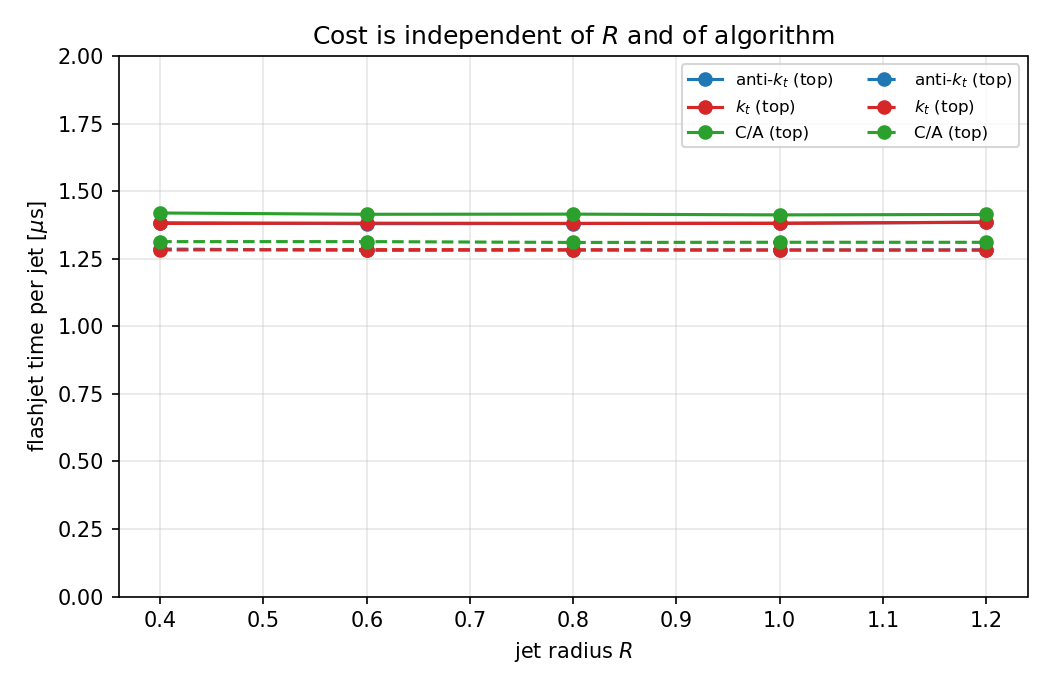
\includegraphics[width=\linewidth]{fig/atlas_R_independence.png}
\end{column}
\begin{column}{0.44\textwidth}
Across $R = 0.4 \rightarrow 1.2$: a \textbf{0.3\,\% spread} over a $3\times$
range in $R$.
\smallskip

$R$ changes \emph{which} pairs merge, not \emph{how many} distances are computed.
\medskip

Across algorithms: \akt, $k_t$ and C/A agree to within $\sim$4\,\% at every
multiplicity.
\medskip

\begin{block}{}
\small $k_t$ and C/A \textbf{cost the same as \akt}.
\end{block}
\end{column}
\end{columns}
\end{frame}

\begin{frame}{Backup --- speedup vs $R$, per algorithm (jet regime) \hfill \realC}
\begin{columns}[T]
\begin{column}{0.5\textwidth}
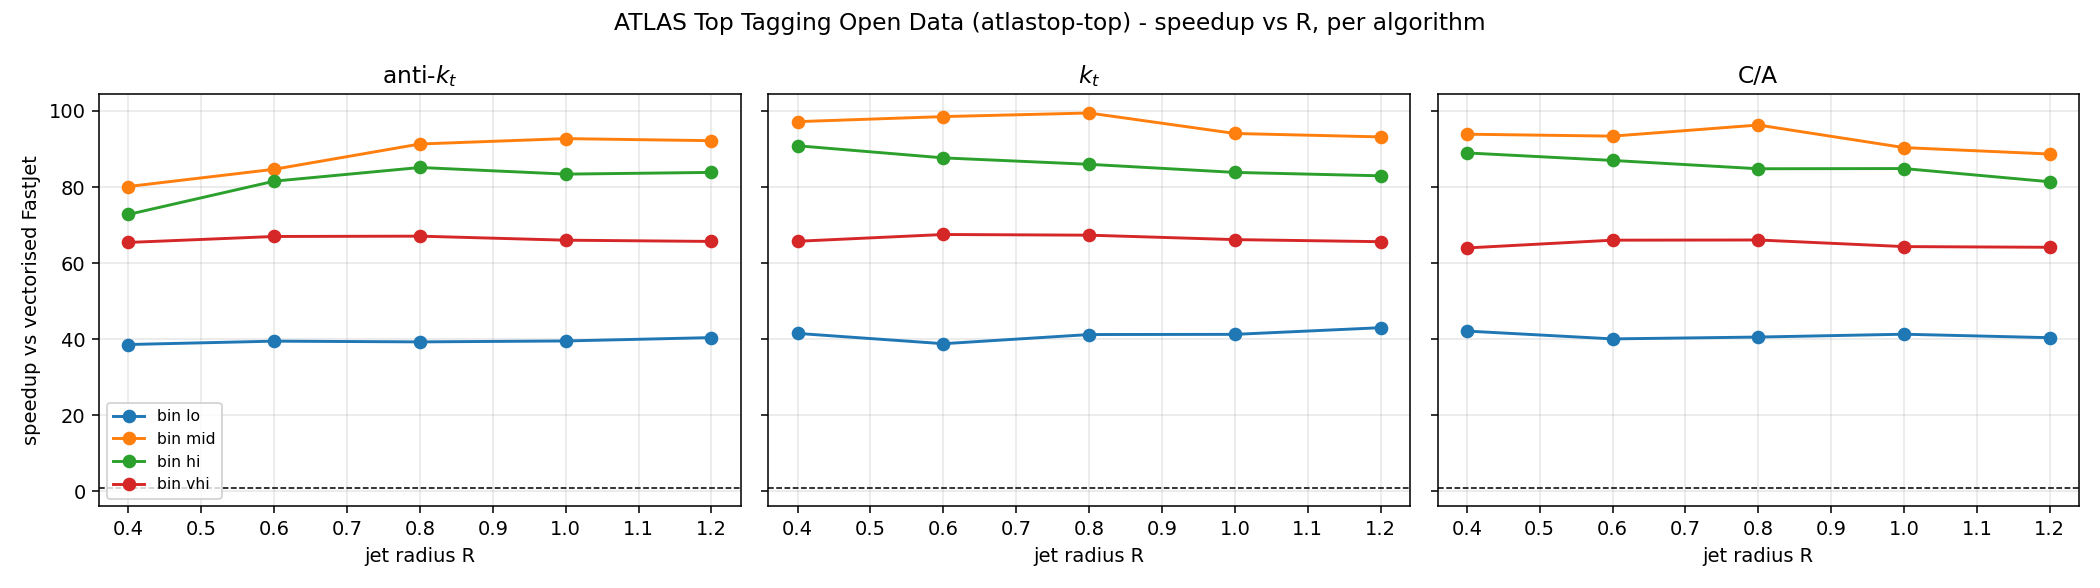
\includegraphics[width=\linewidth]{fig/atlas_radius_scan_atlastop-top.png}\\
\smallnote{boosted top}
\end{column}
\begin{column}{0.5\textwidth}
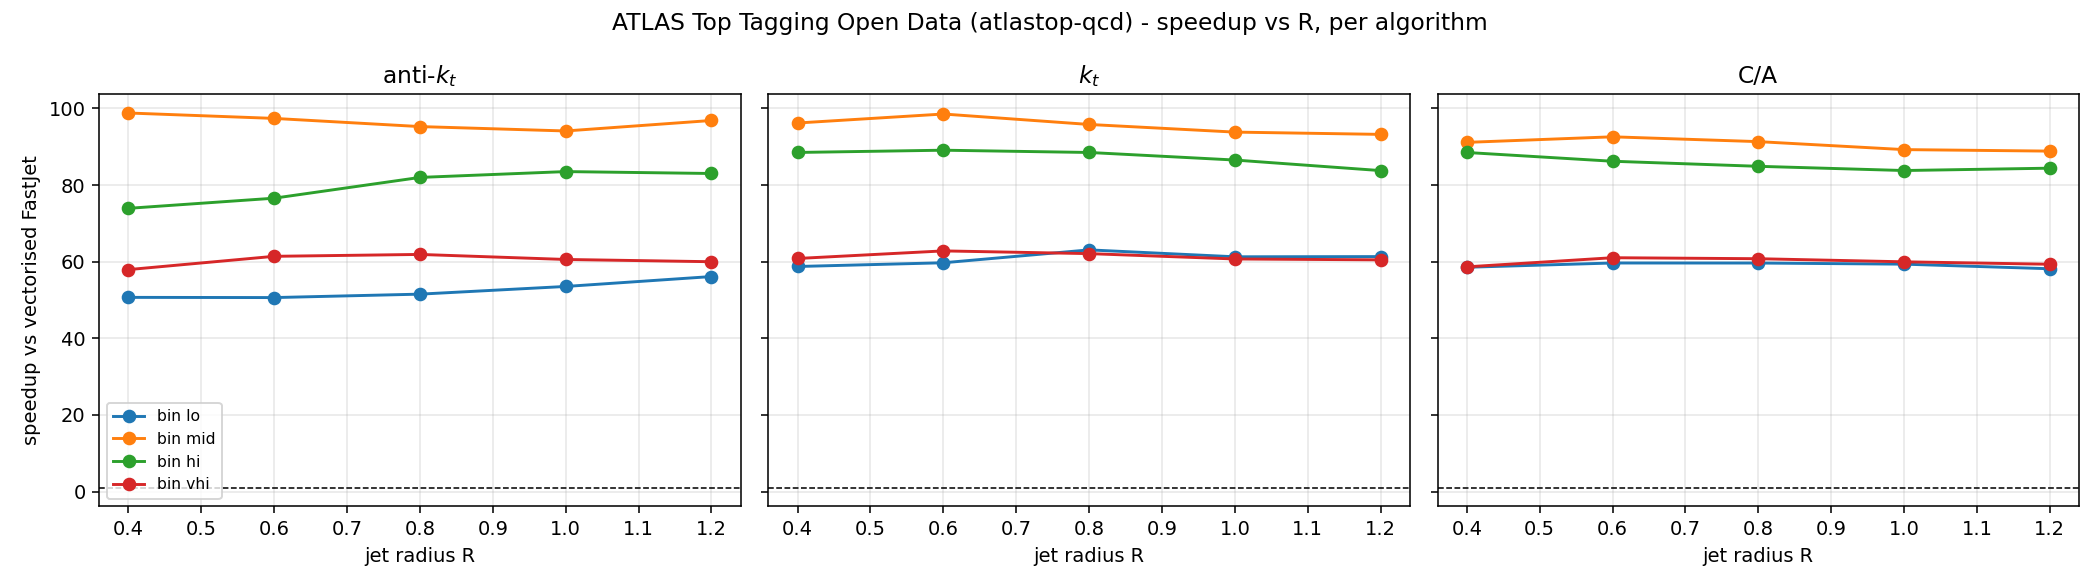
\includegraphics[width=\linewidth]{fig/atlas_radius_scan_atlastop-qcd.png}\\
\smallnote{QCD (light $q/g$)}
\end{column}
\end{columns}
\smallnote{Flat in $R$ for all three algorithms; ordering is by multiplicity bin.}
\end{frame}

\begin{frame}{Backup --- speedup vs multiplicity (jet regime) \hfill \realC}
\begin{columns}[T]
\begin{column}{0.5\textwidth}
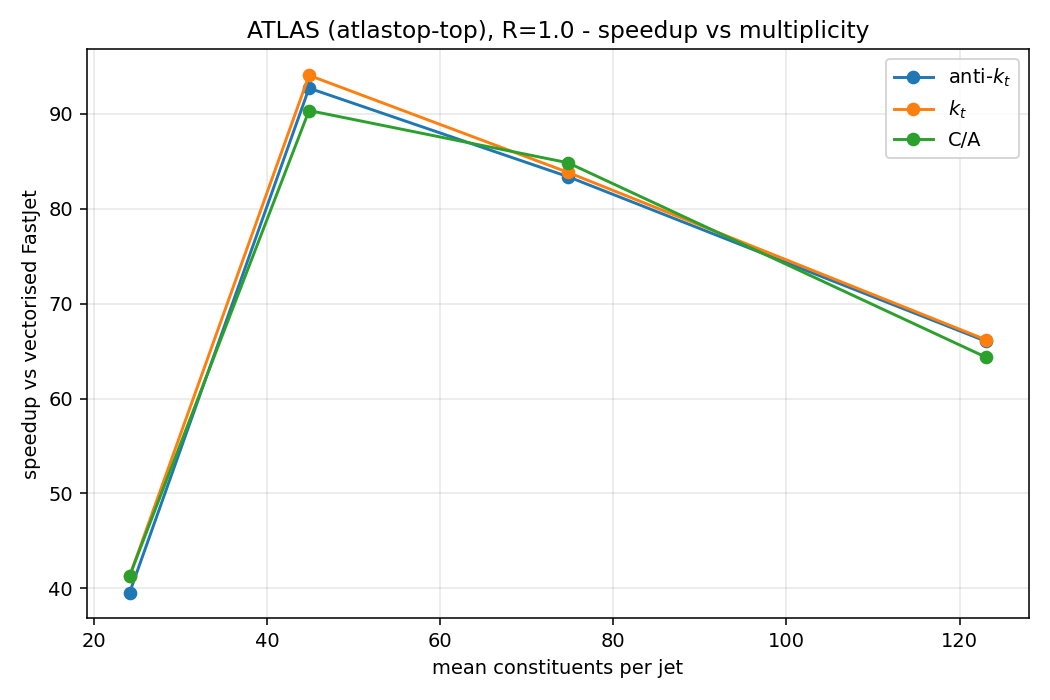
\includegraphics[width=\linewidth]{fig/atlas_multiplicity_atlastop-top.png}\\
\smallnote{boosted top}
\end{column}
\begin{column}{0.5\textwidth}
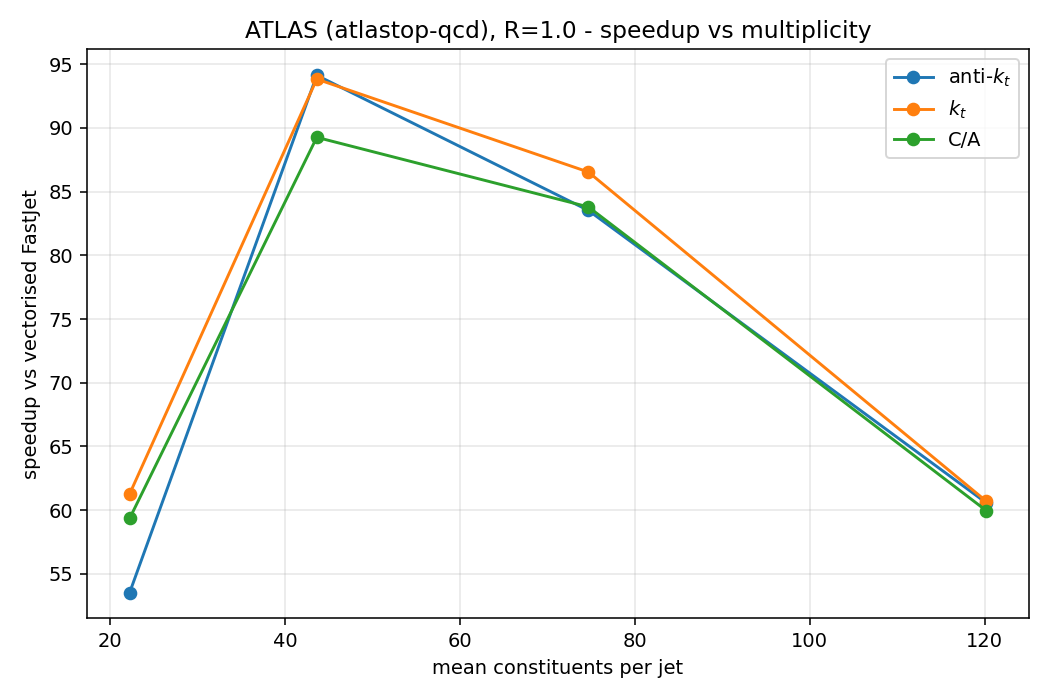
\includegraphics[width=\linewidth]{fig/atlas_multiplicity_atlastop-qcd.png}\\
\smallnote{QCD (light $q/g$)}
\end{column}
\end{columns}
\end{frame}

\begin{frame}{Backup --- the numbers (jet regime)}
\begin{center}
\small
\begin{tabular}{@{}llrrrr@{}}
\toprule
sample & alg & $\langle n\rangle$ & flashjet & FastJet vec. & speedup\\
 & & & [$\mu$s/jet] & [$\mu$s/jet] & \\
\midrule
top & \akt & 24.1 & 0.427 & 16.5 & $39\times$\\
top & \akt & 44.8 & 0.464 & 43.0 & $\mathbf{93\times}$\\
top & C/A  & 74.7 & 1.000 & 84.8 & $85\times$\\
top & C/A  & 123.1 & 2.565 & 165.1 & $64\times$\\
\midrule
qcd & \akt & 22.2 & 0.346 & 17.5 & $51\times$\\
qcd & \akt & 43.6 & 0.463 & 45.7 & $\mathbf{99\times}$\\
qcd & \akt & 74.7 & 1.215 & 89.8 & $74\times$\\
qcd & \akt & 120.2 & 2.673 & 154.9 & $58\times$\\
\bottomrule
\end{tabular}
\end{center}
\medskip
\begin{block}{}
\small \textbf{39--99$\times$} over vectorised FastJet (median $64\times$), with
100\,\% jet-count agreement everywhere. \textbf{One timed unit = one jet},
batched. Benchmarked on an \textbf{NVIDIA V100-class} GPU.
\end{block}
\smallskip
\smallnote{$R=1.0$ rows shown. Against the per-jet FastJet interface the gap is
roughly \emph{two orders of magnitude}.}
\end{frame}

\begin{frame}{Backup --- where the time goes}
\begin{columns}[T]
\begin{column}{0.48\textwidth}
\textbf{Nsight Systems} --- share of GPU time
\smallskip

\begin{tabular}{@{}lrr@{}}
\toprule
kernel & \% GPU & avg/call\\
\midrule
\texttt{\_cluster\_large\_kernel} & \textbf{97.6} & 5.47\,ms\\
\texttt{\_decode\_kernel} & 1.5 & 82\,$\mu$s\\
torch glue & $<1$ & ---\\
\bottomrule
\end{tabular}
\smallskip

\begin{block}{}
\small \textbf{No hidden overhead} --- essentially all the time is real
clustering work, and the memory row of the timeline is empty.
\end{block}
\end{column}
\begin{column}{0.48\textwidth}
\textbf{Nsight Compute} --- hardware counters
\smallskip

\begin{tabular}{@{}lr@{}}
\toprule
metric & value\\
\midrule
DRAM throughput & \textbf{0.02\,\%}\\
Compute (SM) throughput & 15.4\,\%\\
Registers / thread & 168\\
Theoretical occupancy & 18.75\,\%\\
Achieved occupancy & \textbf{6.25\,\%}\\
Waves per SM & \textbf{0.32}\\
\bottomrule
\end{tabular}
\smallskip

\begin{block}{}
\small Not memory- or compute-bound --- the GPU is simply \textbf{not filled}.
\end{block}
\end{column}
\end{columns}
\end{frame}

\begin{frame}{Backup --- the GPU timeline}
\begin{center}
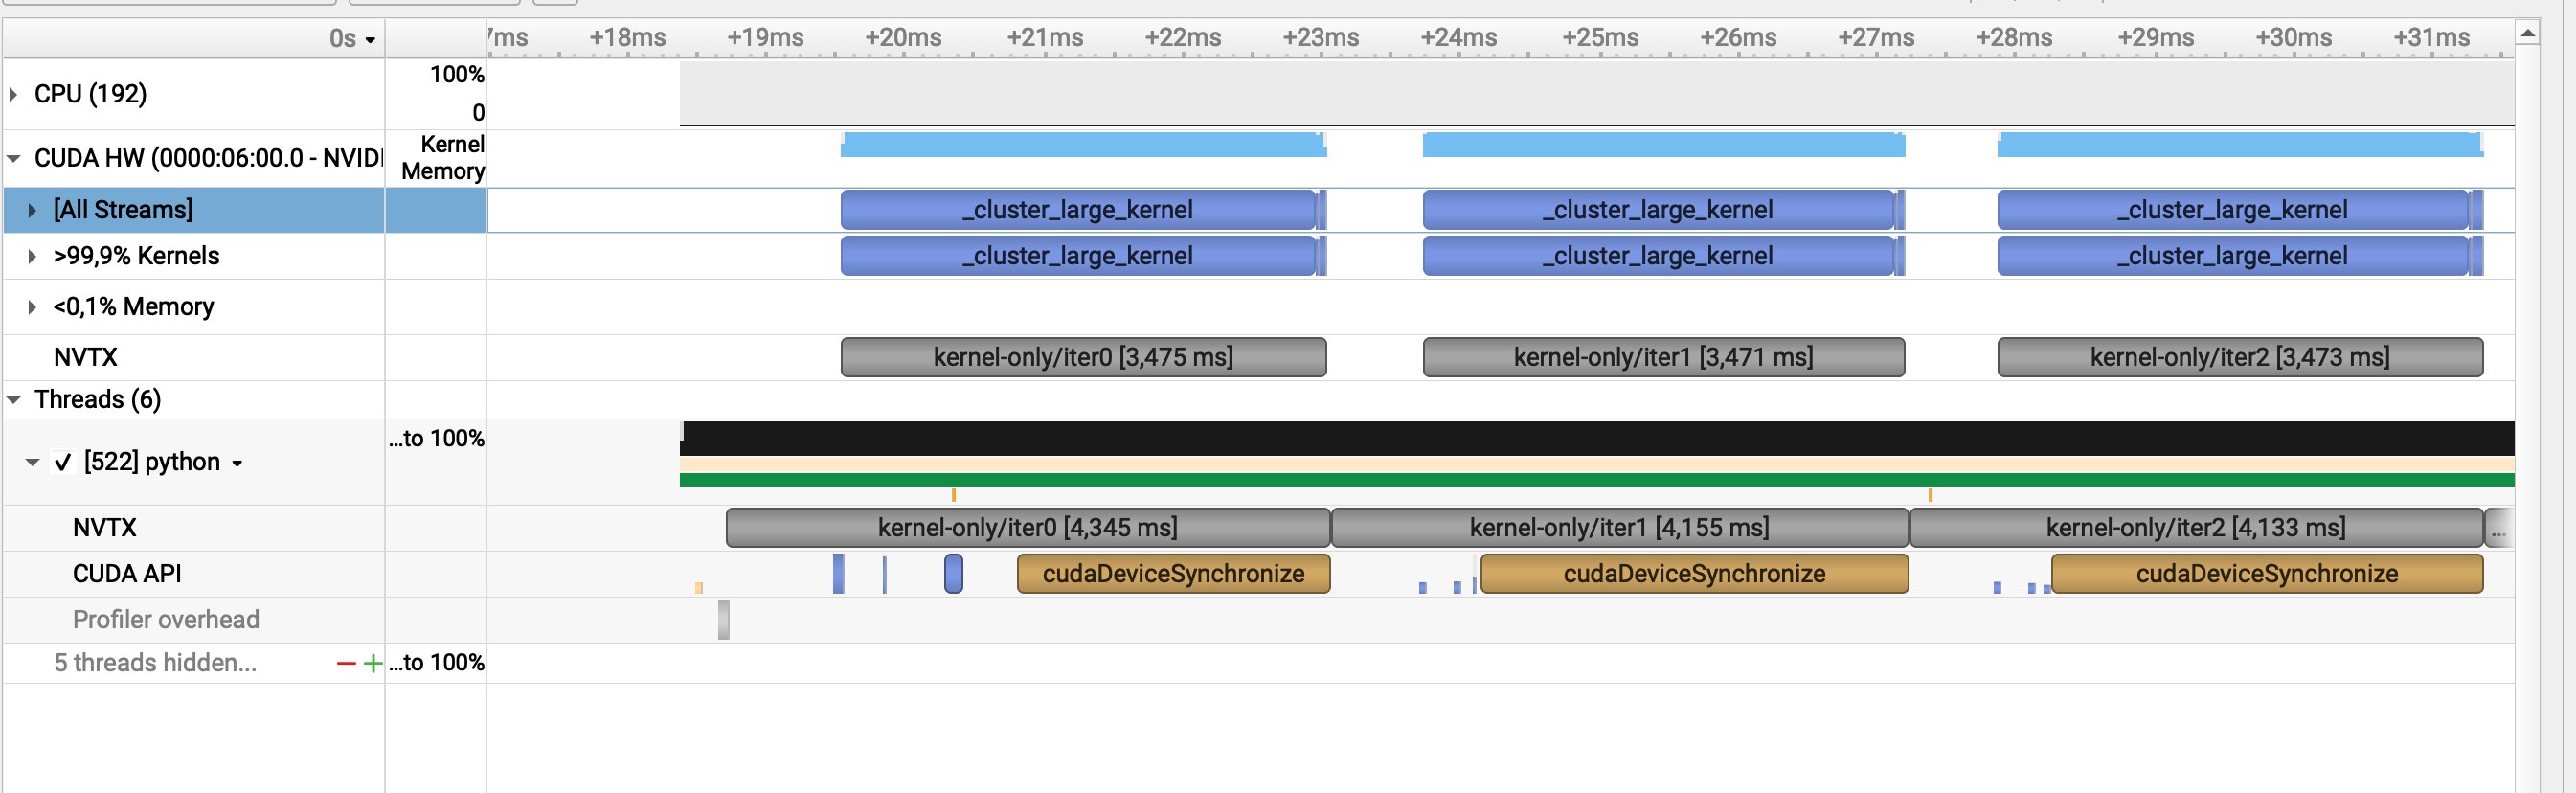
\includegraphics[width=0.80\linewidth]{fig/nsys_timeline_H100.png}
\end{center}
\smallnote{Nsight Systems, three consecutive iterations. Each block is one
clustering call; the tool labels the rows \textbf{``$>$99.9\,\% Kernels''} and
\textbf{``$<$0.1\,\% Memory''}. The kernels run back to back with nothing in
between and the memory row is empty --- no host/device shuffling while
clustering runs. That is what makes the speedup real rather than an artefact of
where the timer was started.}
\end{frame}

\begin{frame}{Backup --- the profiler names the bottleneck}
\begin{columns}[T]
\begin{column}{0.5\textwidth}
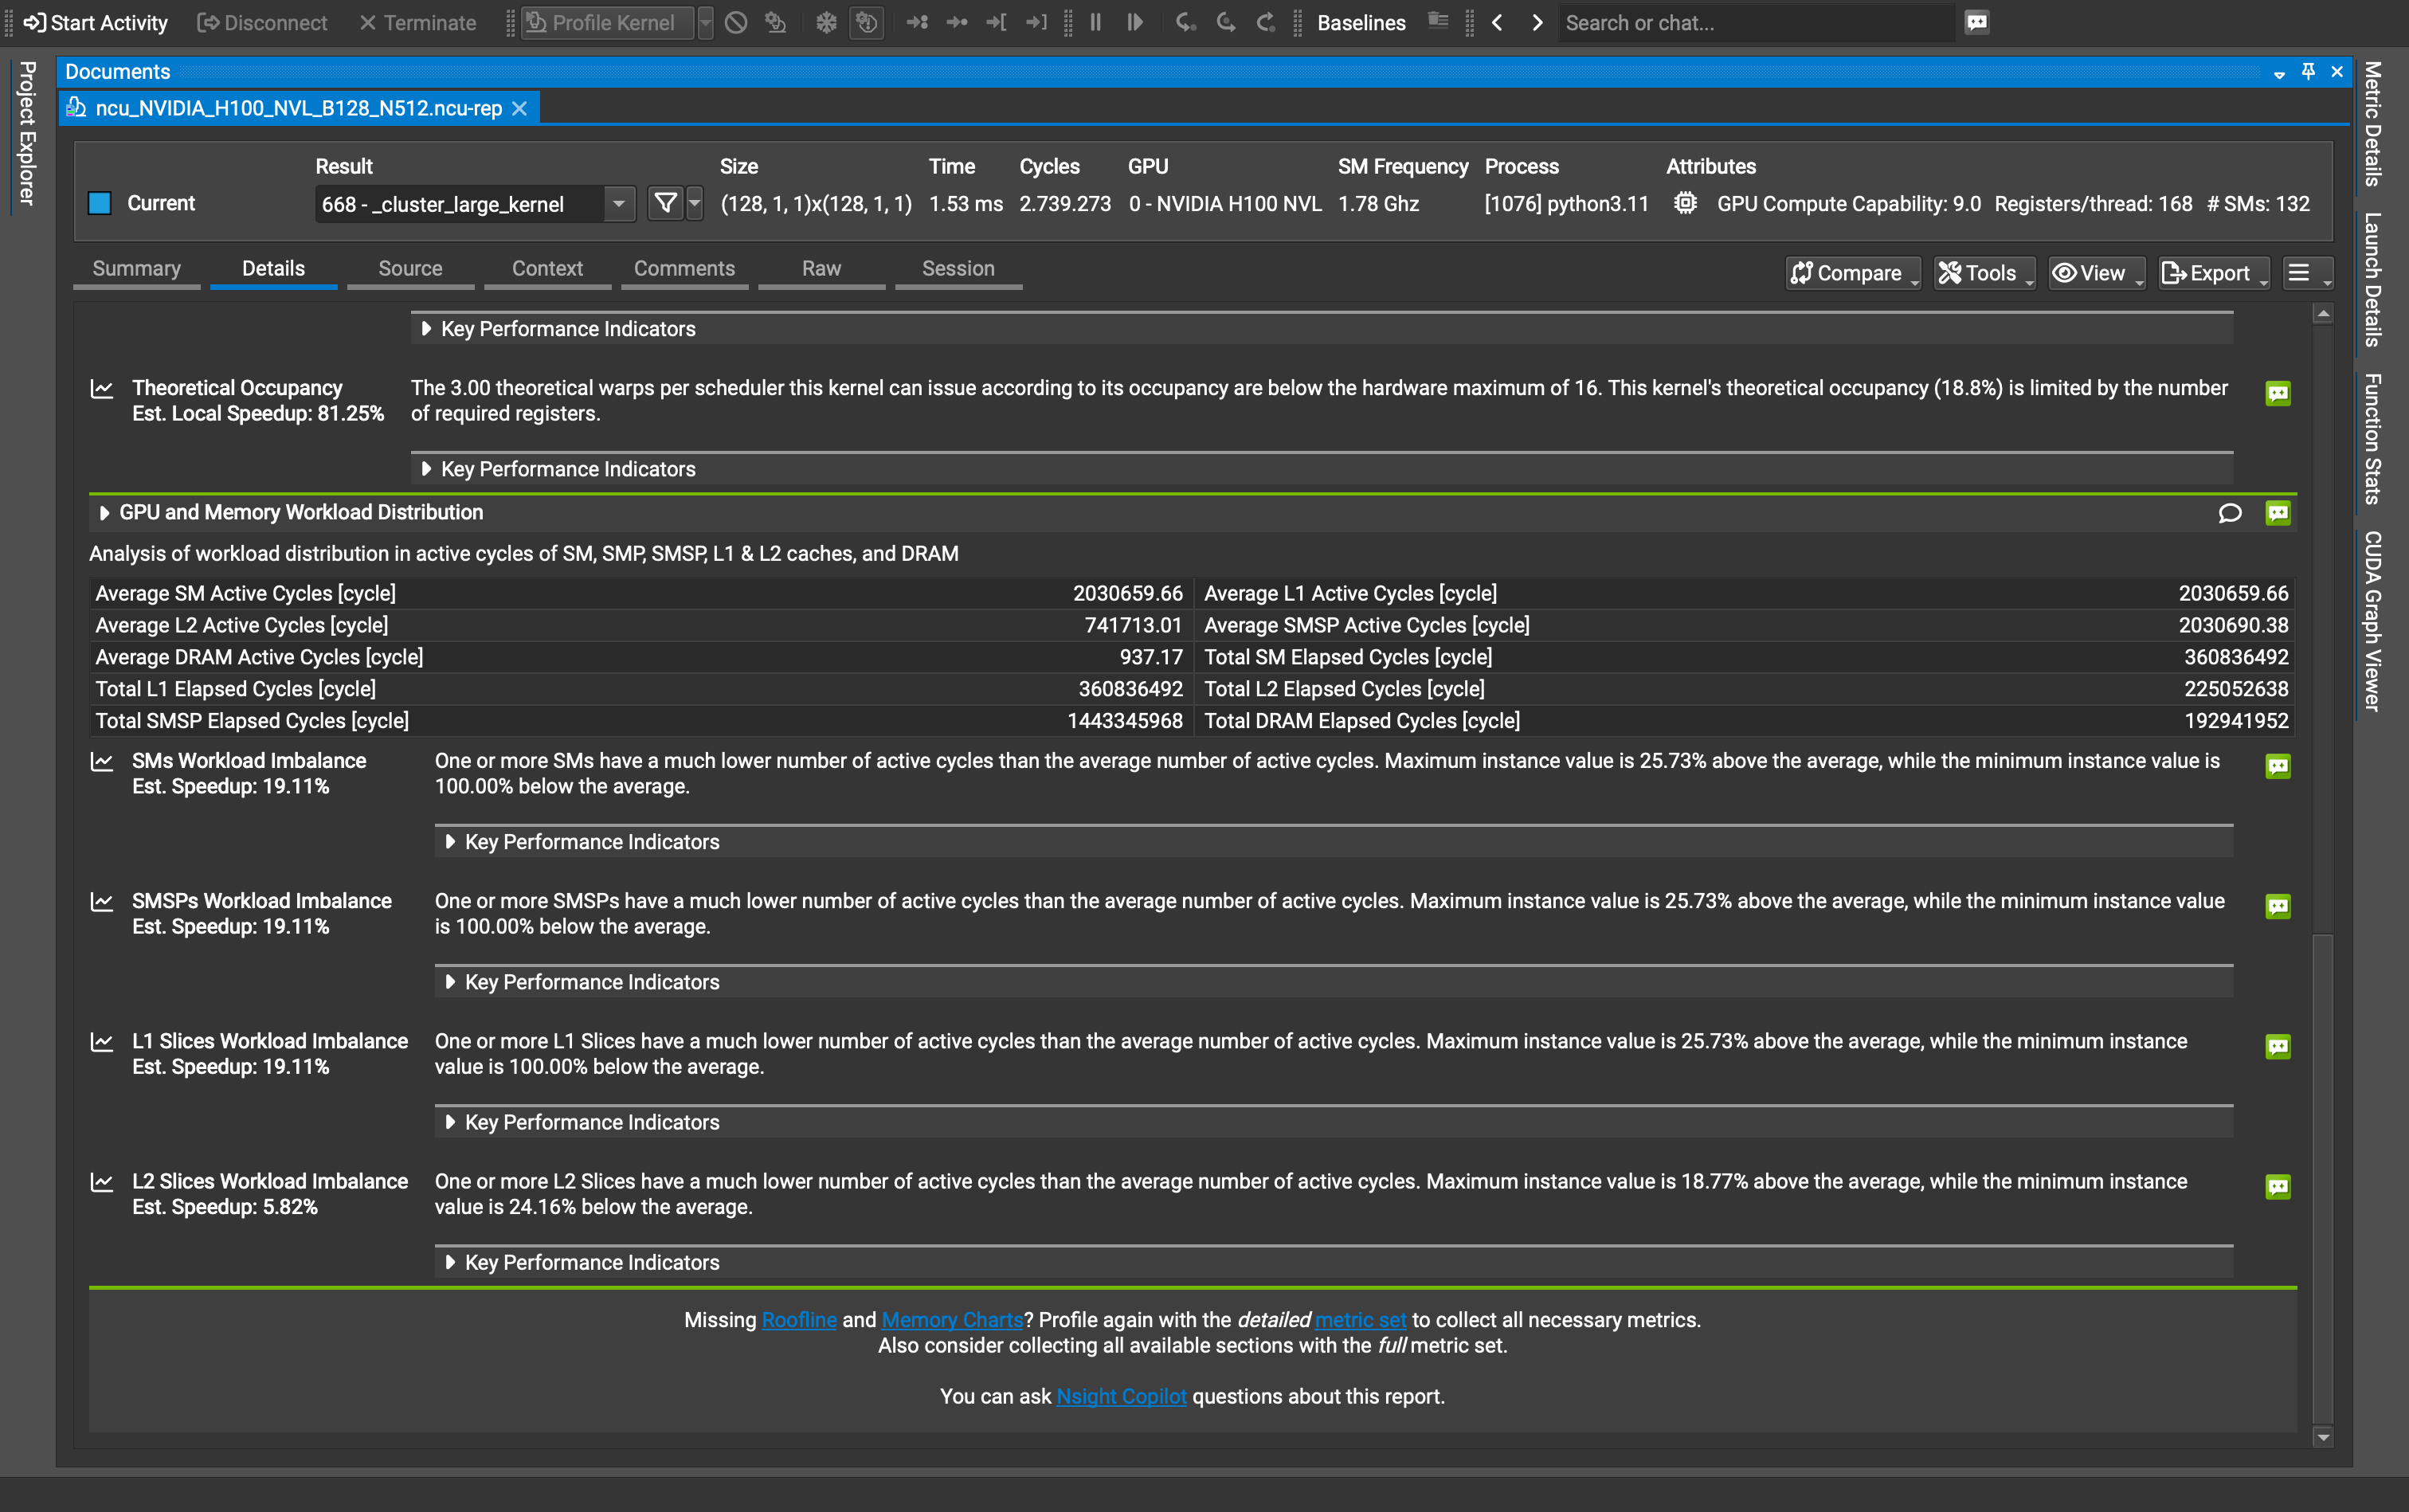
\includegraphics[width=\linewidth]{fig/ncu_workload_imbalance_H100.png}
\end{column}
\begin{column}{0.5\textwidth}
\textbf{The tool's own speedup estimates:}
\smallskip

\begin{tabular}{@{}lr@{}}
\toprule
finding & est.\ speedup\\
\midrule
Theoretical occupancy (registers) & \textbf{81\,\%}\\
Achieved occupancy & 67\,\%\\
SM workload imbalance & 19\,\%\\
\bottomrule
\end{tabular}
\smallskip

\smallnote{\emph{``This kernel grid is too small to fill the available resources
on this device, resulting in only 0.32 full waves across all SMs.''}}
\smallskip

\smallnote{Grid size \textbf{128 blocks} on a \textbf{132-SM} device --- fewer
blocks than the GPU has processors.}
\medskip

\begin{block}{}
\small $\sim$\textbf{1.7--1.8$\times$} more available from launch configuration
and register budget --- \textbf{not} from the algorithm.
\end{block}
\end{column}
\end{columns}
\end{frame}

\begin{frame}{Backup --- occupancy detail}
\begin{columns}[T]
\begin{column}{0.5\textwidth}
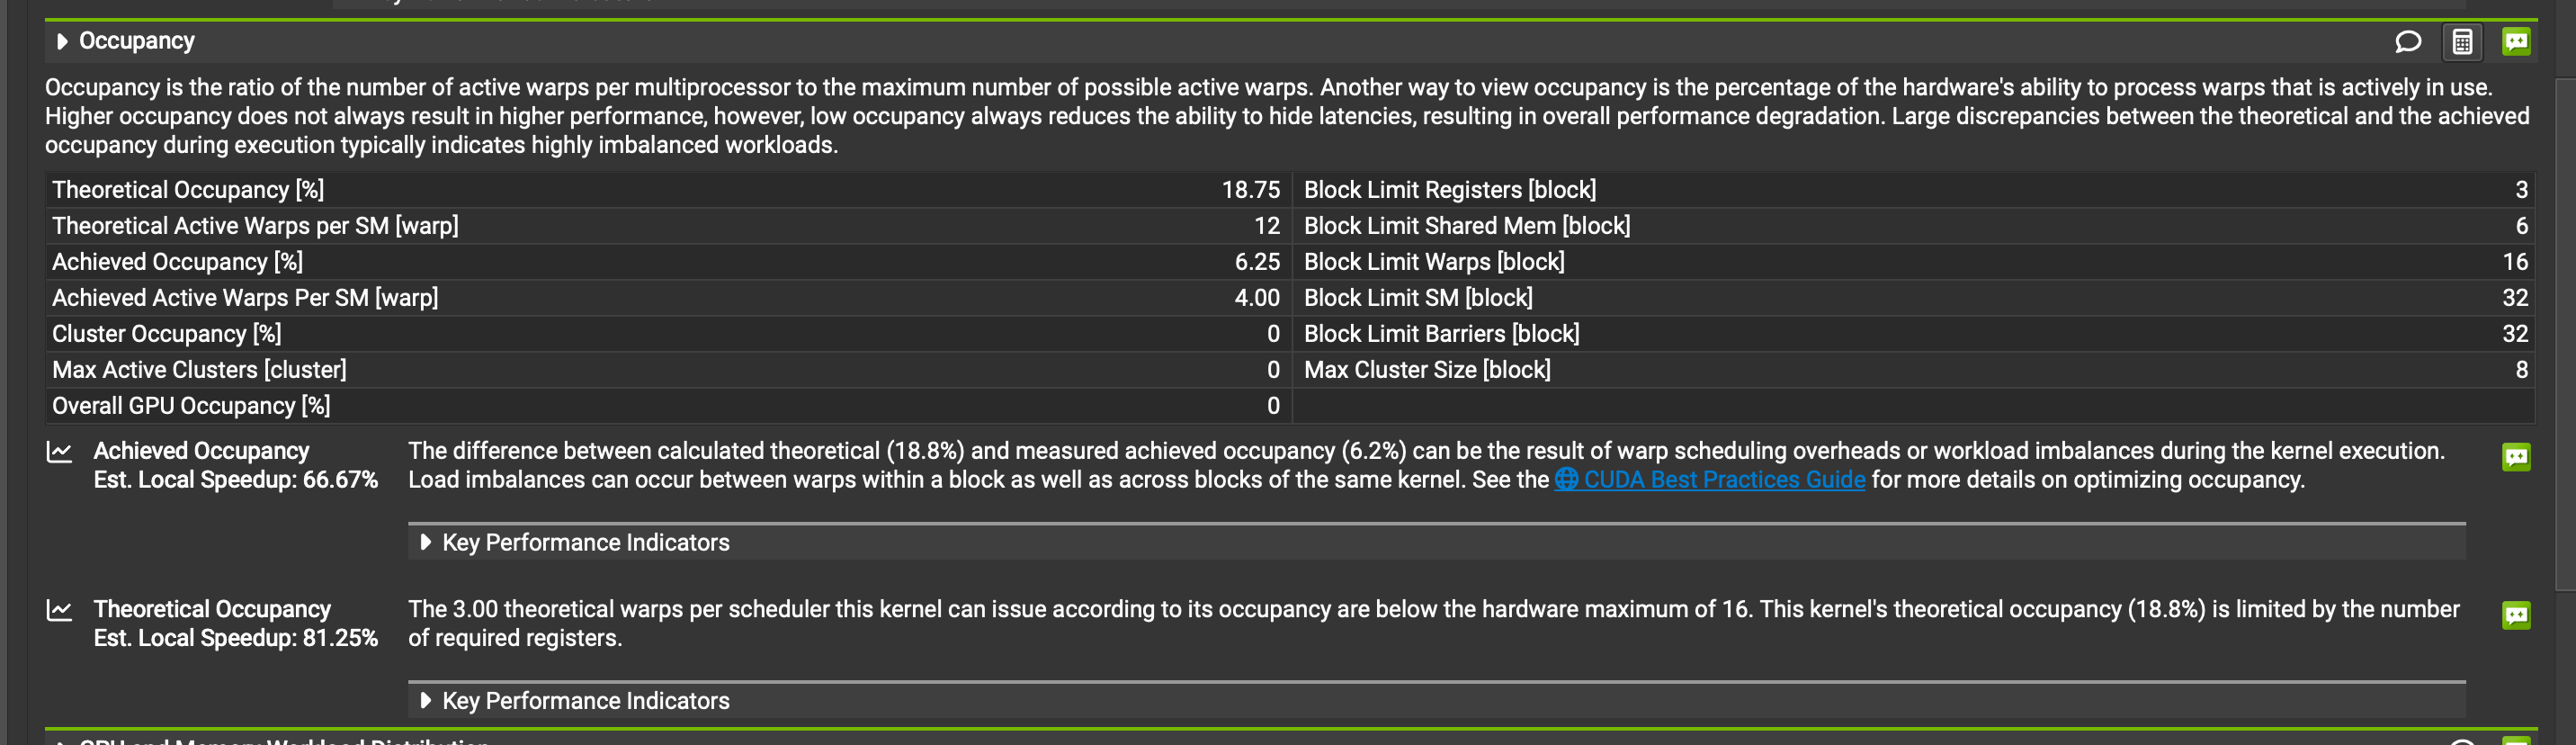
\includegraphics[width=0.95\linewidth]{fig/ncu_occupancy_H100.png}
\end{column}
\begin{column}{0.5\textwidth}
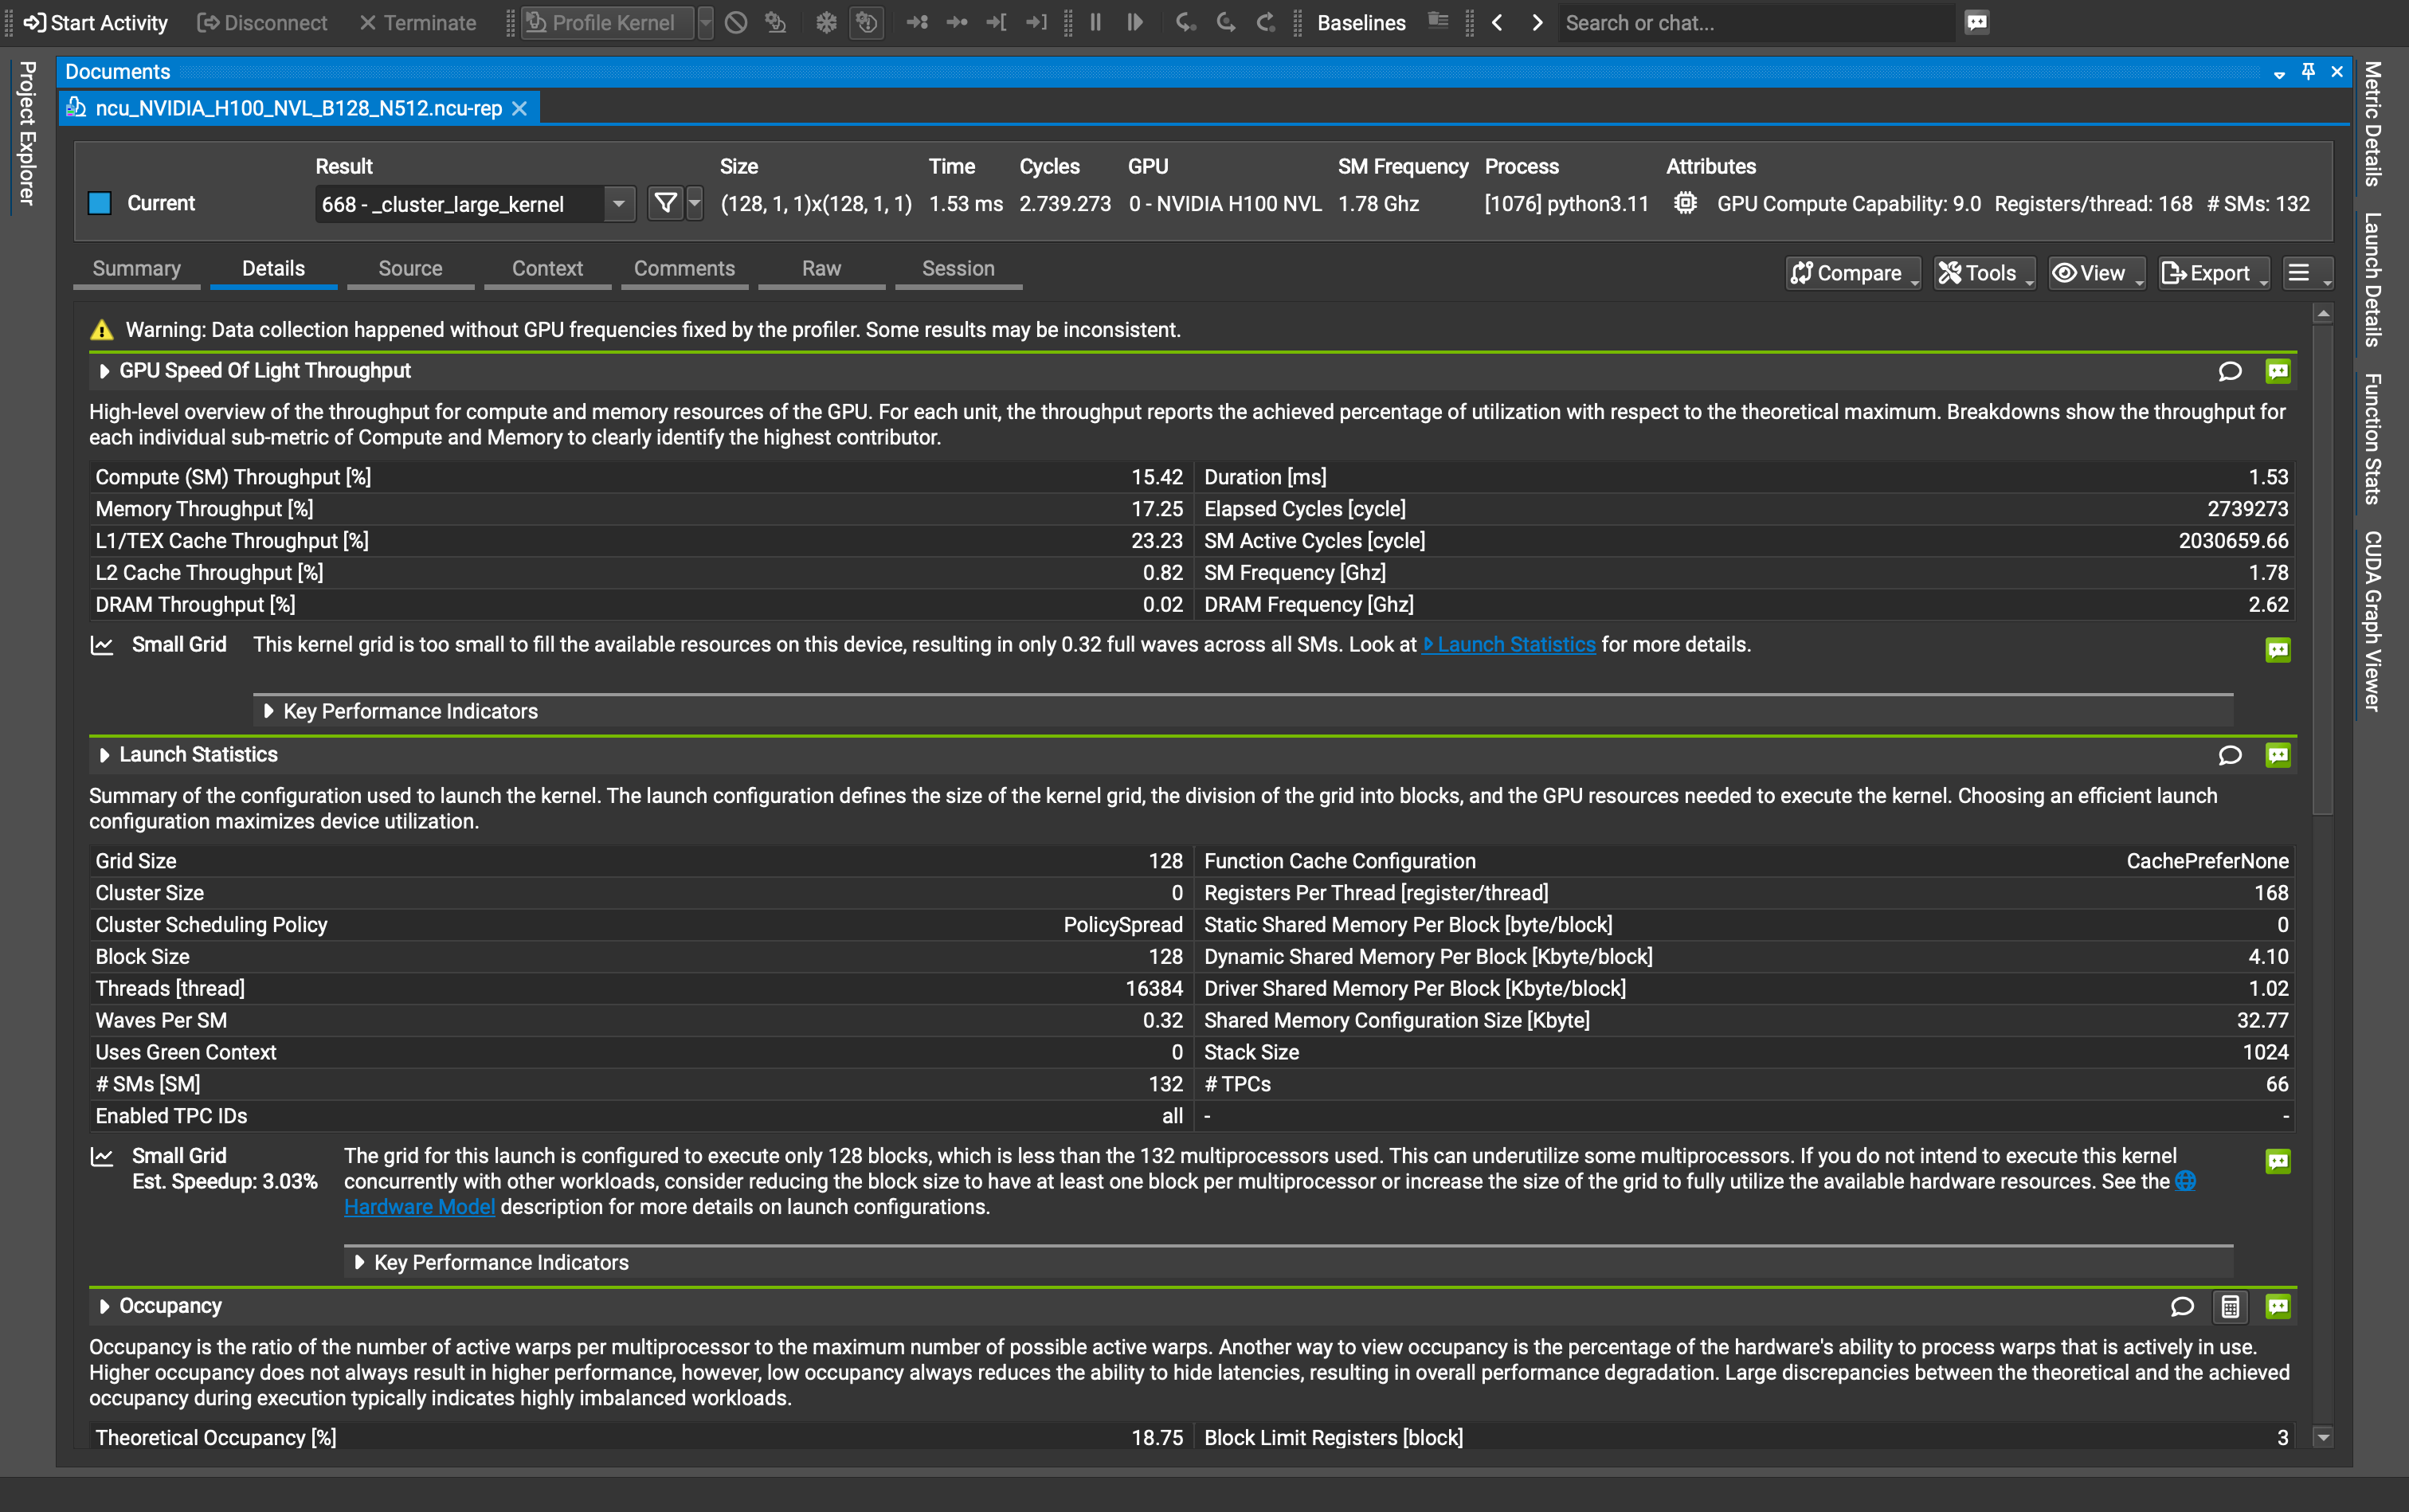
\includegraphics[width=0.95\linewidth]{fig/ncu_details_sol_launch_H100.png}
\end{column}
\end{columns}
\smallnote{Register pressure (168/thread) caps theoretical occupancy at
18.75\,\%; achieved is 6.25\,\%. With 0.32 waves/SM the kernel does not fill the
GPU even once, while DRAM throughput is 0.02\,\% --- this is parallelism
starvation, not a bandwidth problem. Both are configuration inherited from
smaller GPUs, not properties of the algorithm.}
\end{frame}

\begin{frame}{Backup --- more toy closures \hfill \toyB}
\begin{columns}[T]
\begin{column}{0.5\textwidth}
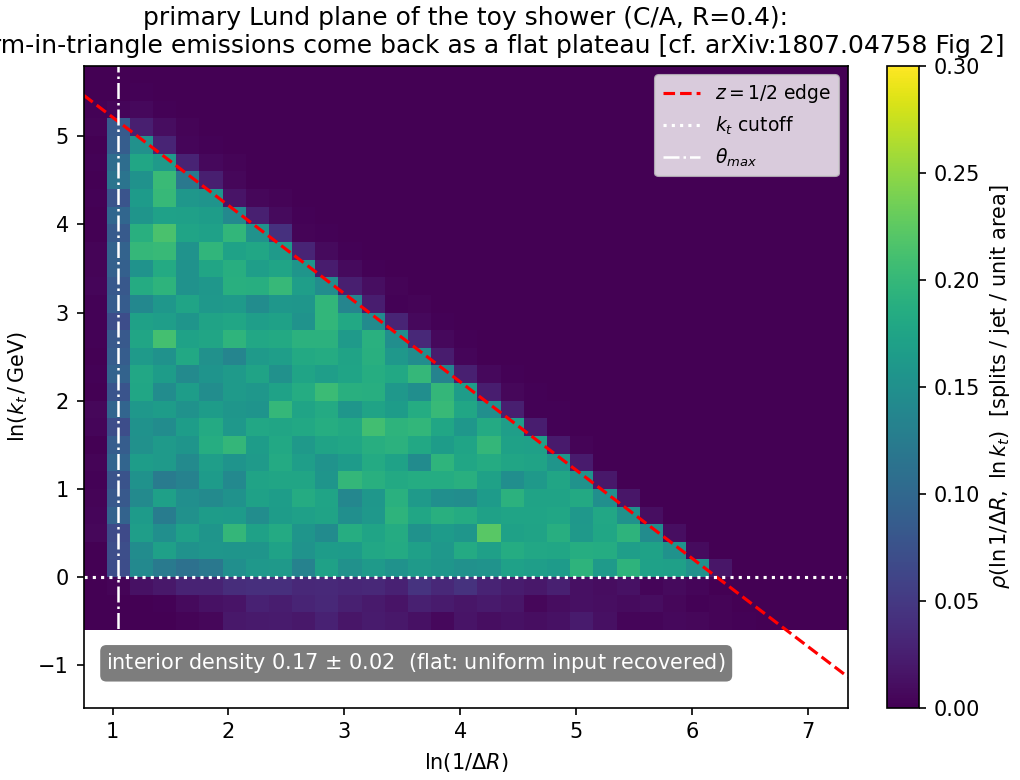
\includegraphics[width=0.95\linewidth]{fig/lund_triangle.png}\\
\smallnote{The Lund plane is populated \textbf{uniformly inside the kinematic
triangle} --- the leading-log expectation.}
\end{column}
\begin{column}{0.5\textwidth}
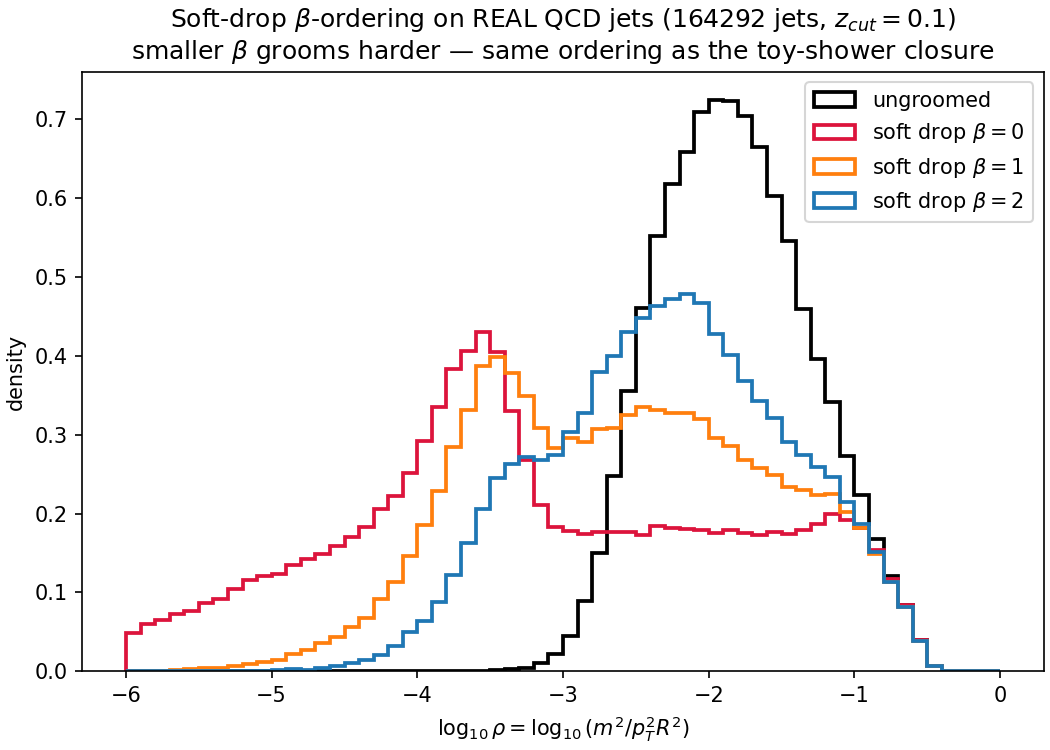
\includegraphics[width=0.95\linewidth]{fig/qcd_beta_family.png}\\
\smallnote{The soft-drop $\beta$-family orders as predicted: larger $\beta$
grooms less.}
\end{column}
\end{columns}
\smallskip
\smallnote{Independent NumPy tree-walks pin every decoder, and the $d$-channel of
the Lund output ties \emph{exactly} to the splitting scales computed separately.}
\end{frame}

\begin{frame}[fragile]{Backup --- Input A: the toy fat jets}
\textbf{Purpose.} QCD vs W is a \emph{known} truth, so any observable that fails
to separate them --- or lands off the analytic curve --- is a real bug.
\medskip

Two single-fat-jet samples at $p_T\!\approx\!500$\,GeV, $R=0.8$:
\begin{itemize}
  \item \textbf{QCD-like}: one hard collinear core (92\,\% of $p_T$,
        $\sigma_{y,\phi}\!=\!0.06$) $+$ soft wide-angle radiation
        (8\,\%, $\sigma\!=\!0.30$)
  \item \textbf{W-like}: two hard prongs with pair mass
        $m=\sqrt{z(1-z)}\,p_T\,\Delta R = 80.4$\,GeV, $z\in[0.30,0.45]$, random
        orientation, $+$ 6\,\% soft contamination
\end{itemize}
\smallskip

Each ``spray'' is $n$ massive pions with exponential $p_T$ fractions:
\begin{Verbatim}[fontsize=\scriptsize,frame=single,rulecolor=\color{fjgray}]
frac = rng.exponential(1., n); frac /= frac.sum()
pt   = pt_total * frac
y, phi = rng.normal(y0, sigma, n), rng.normal(phi0, sigma, n)
mt   = np.sqrt(M_PI**2 + pt**2)
\end{Verbatim}
\smallnote{1500 events per sample. flashjet has \textbf{no event generator} --- it
clusters four-vectors; these toys live in the plot scripts, outside the library.}
\end{frame}

\begin{frame}{Backup --- Input B: the toy parton shower}
A \textbf{primary, fixed-coupling, leading-log} shower: emissions sampled
\textbf{uniformly in the Lund triangle} with density $\bar\alpha$ per unit
$(\ln 1/\theta,\ \ln k_t)$ area, off a hard spine.
\medskip

\begin{center}
$\theta = e^{-u}, \qquad k_t = e^{v}, \qquad z = \dfrac{k_t}{p_{T0}\,\theta}$
\smallskip

keep $v \le \ln(p_{T0}/2) - u$ \ \ (i.e.\ $z\le\tfrac12$), \ \ $k_t > k_t^{\min}$
\end{center}
\medskip

\begin{block}{Why this is the right test}
\small The generator's density is \emph{uniform in the triangle by construction},
so the leading-log predictions --- the $1/z$ form of $z_g$, the $\beta$-ordering
of the groomed mass --- are unambiguous. Landing on them tests the
\textbf{decoders}, not the shower.
\end{block}
\medskip

\textbf{Jet areas} use the anti-$k_t$-paper construction: one hard event plus a
dense grid of \textbf{infinitely soft ghosts} ($p_T=10^{-8}$); the ghosts each
algorithm sweeps up trace its catchment area.
\smallskip

\smallnote{$\bar\alpha = 0.25$, $p_{T0} = 1$\,TeV, $R = 0.4$, 20\,000 showers;
fixed seed, fully re-runnable.}
\end{frame}

\begin{frame}{Backup --- cost of each feature arm}
\begin{columns}[T]
\begin{column}{0.42\textwidth}
\textbf{Wall clock per training step}, relative to the baseline:
\smallskip

\begin{tabular}{@{}lr@{}}
\toprule
arm & cost\\
\midrule
PLuM & \textbf{1.59$\times$}\\
subjet & 1.42$\times$\\
CA5 & 1.22$\times$\\
\bottomrule
\end{tabular}
\smallskip

\smallnote{Features computed live by flashjet inside the loop, on the batch
already resident on the GPU. Parameters: 2.144\,M baseline $\rightarrow$
2.194\,M with the PLuM feature block ($+0.051$\,M).}
\end{column}
\begin{column}{0.58\textwidth}
\begin{block}{}
\small Measured before the GPU-side collation change; the clustering itself is
a small fraction of a step, so these are upper bounds on the true feature cost.
\end{block}
\smallskip

\smallnote{The cost is the reason a null result still matters: if a feature is
free, a null is merely uninteresting --- at \textbf{1.59$\times$} it is a
reason not to use it.}
\end{column}
\end{columns}
\end{frame}

\begin{frame}{Backup --- $W\rightarrow qq$, the fewest-splitting channel}
\begin{columns}[T]
\begin{column}{0.56\textwidth}
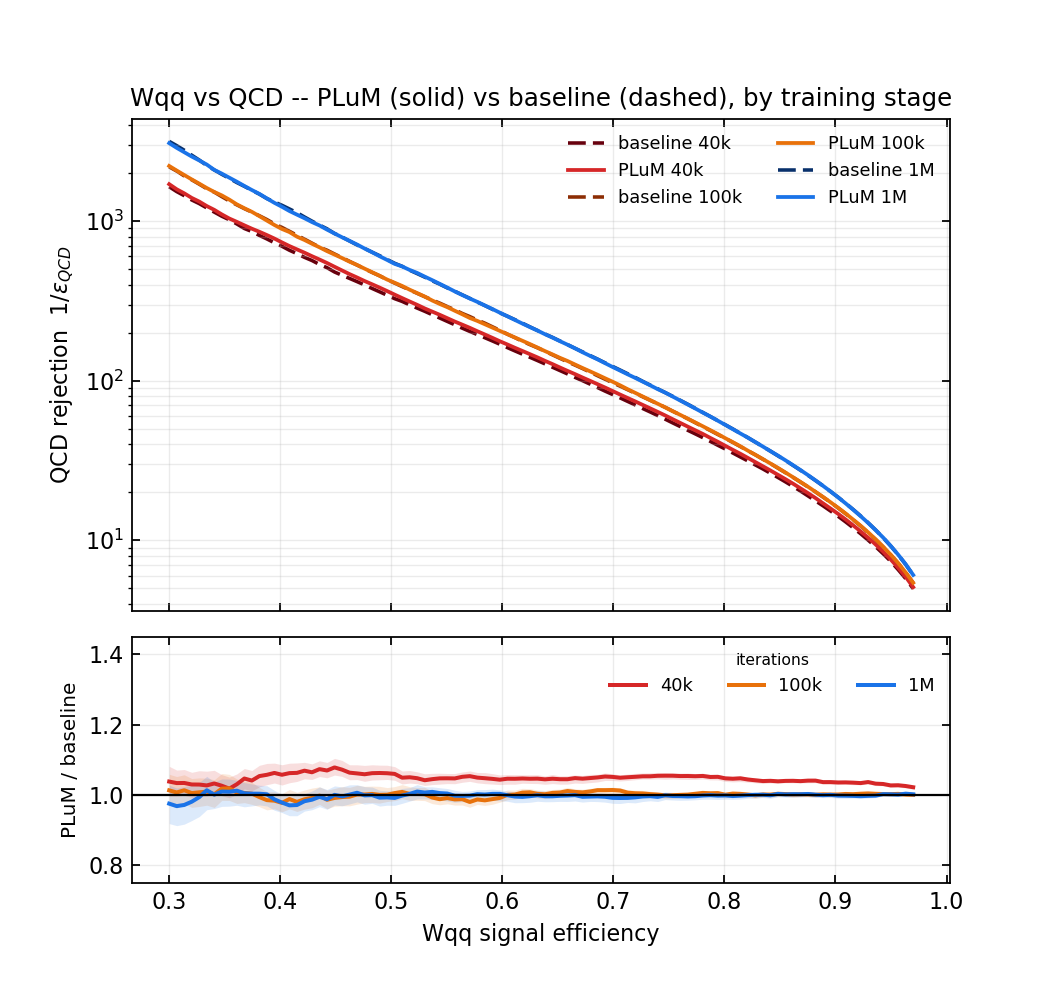
\includegraphics[width=\linewidth,trim=0 18 0 22,clip]{fig/part_rocratio_Wqq.png}
\end{column}
\begin{column}{0.44\textwidth}
\textbf{$W\rightarrow qq$} has the \textbf{fewest} Lund splittings of any
signal class (21.6/jet), yet shows the same early gain.
\smallskip

\begin{block}{}
\small The effect is \textbf{not} confined to complex or $b$-containing jets ---
which is what a decay-structure explanation would predict.
\end{block}
\end{column}
\end{columns}
\end{frame}

\begin{frame}{Backup --- two kinds of validation}
\begin{columns}[T]
\begin{column}{0.5\textwidth}
\begin{block}{First: toys, where truth is known}
\small On generated inputs the \emph{answer} is known analytically --- so any
observable landing off the predicted curve is a real bug, with nothing to hide
behind.
\end{block}
\smallskip
\toyAbody{} --- QCD-like and W-like fat jets\\
\toyBbody{} --- leading-log parton shower
\end{column}
\begin{column}{0.5\textwidth}
\begin{block}{Then: real data, against FastJet}
\small On detector-level jets there is no analytic answer --- so the reference is
\textbf{FastJet on the same events}, and the experiment's own reconstructed jets.
\end{block}
\smallskip
\realCbody{} --- large-$R$ jets and full events
\end{column}
\end{columns}
\vspace{0.8em}
\begin{block}{}
\small The order matters: \textbf{toys first} pins the algorithm against a known
answer; \textbf{real data second} shows it survives detector-level input. A
failure at either stage means something different.
\end{block}
\end{frame}

\begin{frame}{Backup --- the validation ladder}
\begin{center}
\small
\begin{tabular}{@{}llll@{}}
\toprule
\textbf{rung} & \textbf{input} & \textbf{reference} & \textbf{result}\\
\midrule
unit tests & --- & independent NumPy tree-walks & 129 pass, incl.\ GPU paths\\
\addlinespace
\akt{} jet areas & \toyBtxt & the \akt{} paper's own construction & rigid cones,
$\to\pi R^2$\\
$k_t$ substructure & \toyAtxt & known 2-prong vs QCD truth & clean separation\\
soft-drop $z_g$ & \toyBtxt & leading-log $1/z$ prediction & on the curve\\
groomed mass vs $\beta$ & \toyBtxt & Soft Drop Figs.~3--4 & ordering reproduced\\
Lund plane & \toyAtxt & primary-Lund construction & hard split where predicted\\
\addlinespace
jet-by-jet kinematics & \realCtxt & FastJet, same events & 150/150 points,
100\,\% $n_{\rm jets}$\\
full-event clustering & \realCtxt & the experiment's own jets & 100\,\% match,
$\sim$600 clusters/ev\\
\bottomrule
\end{tabular}
\end{center}
\medskip

\begin{block}{}
\small \textbf{Each rung is closed against something independent} --- an
analytic prediction, a separate NumPy implementation, or FastJet itself. No rung
is validated against another part of flashjet.
\end{block}
\end{frame}

\begin{frame}{Backup --- references}
\small
\begin{itemize}\setlength{\itemsep}{3pt}
  \item H.~Qu, C.~Li, S.~Qian, \emph{Particle Transformer for Jet Tagging},
        arXiv:\textbf{2202.03772}. \smallnote{(also the JetClass dataset;
        Zenodo 10.5281/zenodo.6619768)}
  \item L.~Gouskos, B.~Maier, \emph{Particle-Lund Multimodality in Jet Taggers},
        arXiv:\textbf{2605.26821}.
  \item H.~Qu, L.~Gouskos, \emph{Jet tagging via particle clouds}
        \smallnote{(ParticleNet)}, Phys.~Rev.~D \textbf{101} (2020) 056019,
        arXiv:1902.08570.
  \item F.~A.~Dreyer, G.~P.~Salam, G.~Soyez, \emph{The Lund Jet Plane},
        JHEP \textbf{12} (2018) 064, arXiv:1807.04758.
  \item F.~A.~Dreyer, H.~Qu, \emph{Jet tagging in the Lund plane with graph
        networks}, JHEP \textbf{03} (2021) 052, arXiv:2012.08526.
  \item A.~J.~Larkoski, S.~Marzani, G.~Soyez, J.~Thaler, \emph{Soft Drop},
        JHEP \textbf{05} (2014) 146, arXiv:1402.2657.
  \item M.~Cacciari, G.~P.~Salam, G.~Soyez, \emph{The anti-$k_t$ jet clustering
        algorithm}, JHEP \textbf{04} (2008) 063, arXiv:0802.1189; \emph{FastJet
        user manual}, Eur.~Phys.~J.~C \textbf{72} (2012) 1896, arXiv:1111.6097.
  \item S.~Catani, Yu.~L.~Dokshitzer, M.~H.~Seymour, B.~R.~Webber,
        Nucl.~Phys.~B \textbf{406} (1993) 187 \smallnote{($k_t$)};
        Yu.~L.~Dokshitzer \emph{et al.}, hep-ph/9707323 and M.~Wobisch,
        T.~Wengler, hep-ph/9907280 \smallnote{(Cambridge/Aachen)}.
  \item J.~de Favereau \emph{et al.}, \emph{DELPHES 3}, JHEP \textbf{02} (2014)
        057, arXiv:1307.6346.
\end{itemize}
\end{frame}

\begin{frame}{Backup --- the datasets}
All benchmark data is \textbf{ATLAS Open Data} (CC0), read over the public
redirector --- no grid certificate required.
\medskip

\begin{center}
\begin{tabular}{@{}ll@{}}
\toprule
dataset & used for\\
\midrule
ATLAS Top Tagging Open Data & timing + FastJet agreement\\
2020 ATLAS Jet Reconstruction & closure vs the experiment's own jets\\
\bottomrule
\end{tabular}
\end{center}
\medskip

\smallnote{Constituents are calorimeter clusters, massless. Physics closures use
toy showers compared against leading-log analytic predictions, so the prediction
being tested is unambiguous.}
\end{frame}

\end{document}
